% This is the Reed College LaTeX thesis template. Most of the work
% for the document class was done by Sam Noble (SN), as well as this
% template. Later comments etc. by Ben Salzberg (BTS). Additional
% restructuring and APA support by Jess Youngberg (JY).
% Your comments and suggestions are more than welcome; please email
% them to cus@reed.edu
%
% See http://web.reed.edu/cis/help/latex.html for help. There are a
% great bunch of help pages there, with notes on
% getting started, bibtex, etc. Go there and read it if you're not
% already familiar with LaTeX.
%
% Any line that starts with a percent symbol is a comment.
% They won't show up in the document, and are useful for notes
% to yourself and explaining commands.
% Commenting also removes a line from the document;
% very handy for troubleshooting problems. -BTS

% As far as I know, this follows the requirements laid out in
% the 2002-2003 Senior Handbook. Ask a librarian to check the
% document before binding. -SN

%%
%% Preamble
%%
% \documentclass{<something>} must begin each LaTeX document
\documentclass[12pt,twoside]{reedthesis}
% Packages are extensions to the basic LaTeX functions. Whatever you
% want to typeset, there is probably a package out there for it.
% Chemistry (chemtex), screenplays, you name it.
% Check out CTAN to see: http://www.ctan.org/
%%
\usepackage{graphicx,latexsym}
\usepackage{amsmath}
\usepackage{amssymb,amsthm}
\usepackage{longtable,booktabs,setspace}
\usepackage{chemarr} %% Useful for one reaction arrow, useless if you're not a chem major
\usepackage[hyphens]{url}
% Added by CII
\usepackage{hyperref}
\usepackage{lmodern}
\usepackage{float}
\floatplacement{figure}{H}
% End of CII addition
\usepackage{rotating}

% Next line commented out by CII
%%% \usepackage{natbib}
% Comment out the natbib line above and uncomment the following two lines to use the new
% biblatex-chicago style, for Chicago A. Also make some changes at the end where the
% bibliography is included.
%\usepackage{biblatex-chicago}
%\bibliography{thesis}


% Added by CII (Thanks, Hadley!)
% Use ref for internal links
\renewcommand{\hyperref}[2][???]{\autoref{#1}}
\def\chapterautorefname{Chapter}
\def\sectionautorefname{Section}
\def\subsectionautorefname{Subsection}
% End of CII addition

% Added by CII
\usepackage{caption}
\captionsetup{width=5in}
% End of CII addition

% \usepackage{times} % other fonts are available like times, bookman, charter, palatino

% Syntax highlighting #22
  \usepackage{color}
  \usepackage{fancyvrb}
  \newcommand{\VerbBar}{|}
  \newcommand{\VERB}{\Verb[commandchars=\\\{\}]}
  \DefineVerbatimEnvironment{Highlighting}{Verbatim}{commandchars=\\\{\}}
  % Add ',fontsize=\small' for more characters per line
  \usepackage{framed}
  \definecolor{shadecolor}{RGB}{248,248,248}
  \newenvironment{Shaded}{\begin{snugshade}}{\end{snugshade}}
  \newcommand{\AlertTok}[1]{\textcolor[rgb]{0.94,0.16,0.16}{#1}}
  \newcommand{\AnnotationTok}[1]{\textcolor[rgb]{0.56,0.35,0.01}{\textbf{\textit{#1}}}}
  \newcommand{\AttributeTok}[1]{\textcolor[rgb]{0.77,0.63,0.00}{#1}}
  \newcommand{\BaseNTok}[1]{\textcolor[rgb]{0.00,0.00,0.81}{#1}}
  \newcommand{\BuiltInTok}[1]{#1}
  \newcommand{\CharTok}[1]{\textcolor[rgb]{0.31,0.60,0.02}{#1}}
  \newcommand{\CommentTok}[1]{\textcolor[rgb]{0.56,0.35,0.01}{\textit{#1}}}
  \newcommand{\CommentVarTok}[1]{\textcolor[rgb]{0.56,0.35,0.01}{\textbf{\textit{#1}}}}
  \newcommand{\ConstantTok}[1]{\textcolor[rgb]{0.00,0.00,0.00}{#1}}
  \newcommand{\ControlFlowTok}[1]{\textcolor[rgb]{0.13,0.29,0.53}{\textbf{#1}}}
  \newcommand{\DataTypeTok}[1]{\textcolor[rgb]{0.13,0.29,0.53}{#1}}
  \newcommand{\DecValTok}[1]{\textcolor[rgb]{0.00,0.00,0.81}{#1}}
  \newcommand{\DocumentationTok}[1]{\textcolor[rgb]{0.56,0.35,0.01}{\textbf{\textit{#1}}}}
  \newcommand{\ErrorTok}[1]{\textcolor[rgb]{0.64,0.00,0.00}{\textbf{#1}}}
  \newcommand{\ExtensionTok}[1]{#1}
  \newcommand{\FloatTok}[1]{\textcolor[rgb]{0.00,0.00,0.81}{#1}}
  \newcommand{\FunctionTok}[1]{\textcolor[rgb]{0.00,0.00,0.00}{#1}}
  \newcommand{\ImportTok}[1]{#1}
  \newcommand{\InformationTok}[1]{\textcolor[rgb]{0.56,0.35,0.01}{\textbf{\textit{#1}}}}
  \newcommand{\KeywordTok}[1]{\textcolor[rgb]{0.13,0.29,0.53}{\textbf{#1}}}
  \newcommand{\NormalTok}[1]{#1}
  \newcommand{\OperatorTok}[1]{\textcolor[rgb]{0.81,0.36,0.00}{\textbf{#1}}}
  \newcommand{\OtherTok}[1]{\textcolor[rgb]{0.56,0.35,0.01}{#1}}
  \newcommand{\PreprocessorTok}[1]{\textcolor[rgb]{0.56,0.35,0.01}{\textit{#1}}}
  \newcommand{\RegionMarkerTok}[1]{#1}
  \newcommand{\SpecialCharTok}[1]{\textcolor[rgb]{0.00,0.00,0.00}{#1}}
  \newcommand{\SpecialStringTok}[1]{\textcolor[rgb]{0.31,0.60,0.02}{#1}}
  \newcommand{\StringTok}[1]{\textcolor[rgb]{0.31,0.60,0.02}{#1}}
  \newcommand{\VariableTok}[1]{\textcolor[rgb]{0.00,0.00,0.00}{#1}}
  \newcommand{\VerbatimStringTok}[1]{\textcolor[rgb]{0.31,0.60,0.02}{#1}}
  \newcommand{\WarningTok}[1]{\textcolor[rgb]{0.56,0.35,0.01}{\textbf{\textit{#1}}}}

% To pass between YAML and LaTeX the dollar signs are added by CII
\title{Pronouns Good or Bad: Attitudes and Relationships with Gendered Pronouns in Gender-Diverse Undergraduates}
\author{Jade Fung}
% The month and year that you submit your FINAL draft TO THE LIBRARY (May or December)
\date{May 2020}
\division{Philosophy, Religion, Psychology, and Linguistics}
\advisor{Vasiliy Safin}
\institution{Reed College}
\degree{Bachelor of Arts}
%If you have two advisors for some reason, you can use the following
% Uncommented out by CII
% End of CII addition

%%% Remember to use the correct department!
\department{Psychology}
% if you're writing a thesis in an interdisciplinary major,
% uncomment the line below and change the text as appropriate.
% check the Senior Handbook if unsure.
%\thedivisionof{The Established Interdisciplinary Committee for}
% if you want the approval page to say "Approved for the Committee",
% uncomment the next line
%\approvedforthe{Committee}

% Added by CII
%%% Copied from knitr
%% maxwidth is the original width if it's less than linewidth
%% otherwise use linewidth (to make sure the graphics do not exceed the margin)
\makeatletter
\def\maxwidth{ %
  \ifdim\Gin@nat@width>\linewidth
    \linewidth
  \else
    \Gin@nat@width
  \fi
}
\makeatother

%Added by @MyKo101, code provided by @GerbrichFerdinands
\newlength{\cslhangindent}
\setlength{\cslhangindent}{1.5em}
\newenvironment{cslreferences}%
  {\setlength{\parindent}{0pt}%
  \everypar{\setlength{\hangindent}{\cslhangindent}}\ignorespaces}%
  {\par}

\renewcommand{\contentsname}{Table of Contents}
% End of CII addition

\setlength{\parskip}{0pt}

% Added by CII

\providecommand{\tightlist}{%
  \setlength{\itemsep}{0pt}\setlength{\parskip}{0pt}}

\Acknowledgements{
First and foremost, I would like to thank my advisor, Vasiliy, for his patience and continuous support as I changed the scope of my thesis over and over, well into February. Also go us for getting the biggest sample size in a thesis, maybe ever?

Additionally, thank you to Greg for helping me figure out how to use magic i.e.~use PCA, which I think most people will probably end up thinking is magic but whatever. It's just an undergraduate thesis. Sorry that I stopped coming to class but still came to your office hour for thesis help haha.

I would also like to thank my roommate and best friend Isaac for revealing to me the true, nefarious purpose of homosexuality, which I am now sworn to take to the grave without telling another soul. Also thanks for cooking me dinner almost every day for that two week period where I didn't go to class and just worked on my thesis and talked about girls. You are the truly the best fag a dyke could ask for.

Also, thank you to my pal of pals and thesis desk partner Lou, who, regardless of the pronouns I was in to, was always by side and down to banter in a variety of accents and codes for four straight years! Four years! Alright! Cheerio!

Thank you to Riley who accompanied me in IRL life, and then via FaceTime as the pandemic fell over Oregon, in my descent into madness as I began realizing that, while the semester was ending, the completion thesis was not. You're quite funny \emph{very} pretty, \emph{even} for a tranny. See you tomorrow.

Thank you to Jay who transitioned from cycling buddy to R Markdown buddy as you graduated and I started thesis. Hopefully we can detransition soon.

Thank you to all of my dear gender-diverse feminists: Io, Schuster, Nell, and Zoe. While I don't think we actually settled on a definition of ``gender diverse,'' I'm glad that we were able to exercise that term enough for me to feel confident using it in my thesis title and never define it in the text.

Thank you to Paulina, whose overflowing passion for fancy liquids and weird modern classical music knows no geographical bounds i.e.~not Oregon i.e.~Chicago. Let's do that again sometime.

Thank you to Vivek, whose camradery in high quality music and appreciation for Paul was a continuous sorce of joy over the years. It's a shame you chose the worse major---neuroscience---so we'll never truly be on equal footing, but I see you and I appreciate you. Also thanks for your short-lived TA role with Beef Tip helping us teach Ophelia to press the lever on her \emph{other} right.

Thank you to Saxton, who \emph{also} sat with me on the lawn as the world switched up it vibes. Because I got an extension on my thesis, I have the privlege of ripping your acknowledgement text for mine.

Thank you to Saga who entertained bit after bit in the PARC when they really had no choice because they were at work. Also thank you for finally revealing the author's rhetorical purpose in your thesis. While I don't personally grasp what ``g*y s*x'' means, I trust you and the personal significance it holds for you.

Thank you to my dear Reed College dolls: Mia, Beatrice, and Winn. How very feminist of us to queer higher-ed and our small liberal arts college in the Portland Northwest by transitioning while studying. Stunning.

Thank you to the REED COLLEGE LOW BRASS SECTION! We really brought that Reed College sound for FOUR YEARS in a row! Don't you all remember four years ago? With Yuan? Anyone? Thank you to all of the Low Brass underclassmen, Henry, Jon, and Gloria, who bought Ryen and I pizza seemingly every night this semester until the 2019--20 coronavirus pandemic put a halt to all of that.

Thank you to Kristin, whose continuous encouragement, support, and interest in my work in and out of the mLab pushed me to new levels.

Thank you to Dr.~Kelly ``Preisdent of Solid Air'' Chacón PhD Esq., whose, frankly, \emph{rediculous} tollerance of my bits blossomed into a wonderful friendship. In your own words, I now know neither physics nor chemistry. But, I have a friend. Additionally, thank you to Luke and Pax for your impressive and continuous commitment to the bit. Also hi Alex!

Thank you also to everyone who attended the Tuesday Transgender injection Zoom meeting, including Benjamin, Shaan, Iris, Maddox, Beq, Winn, and August. How cool of us to be transgender in the time of COVID.

Thank you to the many people who sent me kind words of encouragement when I was frustrated that the pronouns just weren't adding up. There are too many of you to thank, but I appreciate all of you and you help lift this thesis to what it is today.

Thank you KDFC, for continuously entertaining me from 8:30am-ish to 10-10:30-ish every day for the past four years. I have but one small suggestion: please replace the Classical Commuter Quiz and the Musical Blind Date with additional segments of Mozart in the Morning, they are not necessary and Mozart is better. Thanks.

And most importantly, to Tuesday, as in the day of the week. You were always there for me. Truly you make the natiform indent in meaning that falls between Monday and Wednesday. Thanks, Tuesday.
}

\Dedication{
I would like to dedicate this thesis to my mother, whose continuous support in every part of my life has made this thesis and so much more possible. I love you, mom.
}

\Preface{

}

\Abstract{
Gendered third-person pronouns such as ``she'' are used to refer to people in a manner that is congruent with their gender. For many cisgender people, this is an unquestioned truth. However, for transgender and non-binary people, correct use of one's gendered pronouns can be as important as one's chosen name. Transgender literature has not yet examined relationships with gendered pronouns in detail. In this study, we developed a survey about relationships with and attitudes towards gendered pronouns. Additionally, two previously validated measures of gender congruence and active support of transgender people were included in the survey. This was administered to undergraduates at Reed College, where a significant proportion of the student body is gender non-confirming, transgender, and non-binary. The sample also includes cisgender people. We found that pronouns are a poor signifier of gender, and that people of all genders use many different combinations of pronouns. Furthermore, we found that relationships to pronouns is complicated and multivariate. Using primary component analysis, we found that a significant proportion of the data can be explained by how deeply one is affected by cisnormativity---the systematic privileging of cisgender people. Ultimately, relationships to pronouns are complicated and deeply individual. We also found that cis people generally lag behind trans and non-binary people in supporting trans people. One concrete way that cis people can support their trans peers is by initiating the sharing of pronouns.
}

	\usepackage{booktabs}
 \usepackage{longtable}
 \usepackage{array}
 \usepackage{multirow}
 \usepackage{wrapfig}
 \usepackage{float}
 \usepackage{colortbl}
 \usepackage{pdflscape}
 \usepackage{tabu}
 \usepackage{threeparttable}
 \usepackage{threeparttablex}
 \usepackage[normalem]{ulem}
 \usepackage{makecell}
 \usepackage{xcolor}
% End of CII addition
%%
%% End Preamble
%%
%
\begin{document}

% Everything below added by CII
  \maketitle

\frontmatter % this stuff will be roman-numbered
\pagestyle{empty} % this removes page numbers from the frontmatter
  \begin{acknowledgements}
    First and foremost, I would like to thank my advisor, Vasiliy, for his patience and continuous support as I changed the scope of my thesis over and over, well into February. Also go us for getting the biggest sample size in a thesis, maybe ever?

    Additionally, thank you to Greg for helping me figure out how to use magic i.e.~use PCA, which I think most people will probably end up thinking is magic but whatever. It's just an undergraduate thesis. Sorry that I stopped coming to class but still came to your office hour for thesis help haha.

    I would also like to thank my roommate and best friend Isaac for revealing to me the true, nefarious purpose of homosexuality, which I am now sworn to take to the grave without telling another soul. Also thanks for cooking me dinner almost every day for that two week period where I didn't go to class and just worked on my thesis and talked about girls. You are the truly the best fag a dyke could ask for.

    Also, thank you to my pal of pals and thesis desk partner Lou, who, regardless of the pronouns I was in to, was always by side and down to banter in a variety of accents and codes for four straight years! Four years! Alright! Cheerio!

    Thank you to Riley who accompanied me in IRL life, and then via FaceTime as the pandemic fell over Oregon, in my descent into madness as I began realizing that, while the semester was ending, the completion thesis was not. You're quite funny \emph{very} pretty, \emph{even} for a tranny. See you tomorrow.

    Thank you to Jay who transitioned from cycling buddy to R Markdown buddy as you graduated and I started thesis. Hopefully we can detransition soon.

    Thank you to all of my dear gender-diverse feminists: Io, Schuster, Nell, and Zoe. While I don't think we actually settled on a definition of ``gender diverse,'' I'm glad that we were able to exercise that term enough for me to feel confident using it in my thesis title and never define it in the text.

    Thank you to Paulina, whose overflowing passion for fancy liquids and weird modern classical music knows no geographical bounds i.e.~not Oregon i.e.~Chicago. Let's do that again sometime.

    Thank you to Vivek, whose camradery in high quality music and appreciation for Paul was a continuous sorce of joy over the years. It's a shame you chose the worse major---neuroscience---so we'll never truly be on equal footing, but I see you and I appreciate you. Also thanks for your short-lived TA role with Beef Tip helping us teach Ophelia to press the lever on her \emph{other} right.

    Thank you to Saxton, who \emph{also} sat with me on the lawn as the world switched up it vibes. Because I got an extension on my thesis, I have the privlege of ripping your acknowledgement text for mine.

    Thank you to Saga who entertained bit after bit in the PARC when they really had no choice because they were at work. Also thank you for finally revealing the author's rhetorical purpose in your thesis. While I don't personally grasp what ``g*y s*x'' means, I trust you and the personal significance it holds for you.

    Thank you to my dear Reed College dolls: Mia, Beatrice, and Winn. How very feminist of us to queer higher-ed and our small liberal arts college in the Portland Northwest by transitioning while studying. Stunning.

    Thank you to the REED COLLEGE LOW BRASS SECTION! We really brought that Reed College sound for FOUR YEARS in a row! Don't you all remember four years ago? With Yuan? Anyone? Thank you to all of the Low Brass underclassmen, Henry, Jon, and Gloria, who bought Ryen and I pizza seemingly every night this semester until the 2019--20 coronavirus pandemic put a halt to all of that.

    Thank you to Kristin, whose continuous encouragement, support, and interest in my work in and out of the mLab pushed me to new levels.

    Thank you to Dr.~Kelly ``Preisdent of Solid Air'' Chacón PhD Esq., whose, frankly, \emph{rediculous} tollerance of my bits blossomed into a wonderful friendship. In your own words, I now know neither physics nor chemistry. But, I have a friend. Additionally, thank you to Luke and Pax for your impressive and continuous commitment to the bit. Also hi Alex!

    Thank you also to everyone who attended the Tuesday Transgender injection Zoom meeting, including Benjamin, Shaan, Iris, Maddox, Beq, Winn, and August. How cool of us to be transgender in the time of COVID.

    Thank you to the many people who sent me kind words of encouragement when I was frustrated that the pronouns just weren't adding up. There are too many of you to thank, but I appreciate all of you and you help lift this thesis to what it is today.

    Thank you KDFC, for continuously entertaining me from 8:30am-ish to 10-10:30-ish every day for the past four years. I have but one small suggestion: please replace the Classical Commuter Quiz and the Musical Blind Date with additional segments of Mozart in the Morning, they are not necessary and Mozart is better. Thanks.

    And most importantly, to Tuesday, as in the day of the week. You were always there for me. Truly you make the natiform indent in meaning that falls between Monday and Wednesday. Thanks, Tuesday.
  \end{acknowledgements}

  \hypersetup{linkcolor=black}
  \setcounter{tocdepth}{2}
  \tableofcontents

  \listoftables

  \listoffigures
  \begin{abstract}
    Gendered third-person pronouns such as ``she'' are used to refer to people in a manner that is congruent with their gender. For many cisgender people, this is an unquestioned truth. However, for transgender and non-binary people, correct use of one's gendered pronouns can be as important as one's chosen name. Transgender literature has not yet examined relationships with gendered pronouns in detail. In this study, we developed a survey about relationships with and attitudes towards gendered pronouns. Additionally, two previously validated measures of gender congruence and active support of transgender people were included in the survey. This was administered to undergraduates at Reed College, where a significant proportion of the student body is gender non-confirming, transgender, and non-binary. The sample also includes cisgender people. We found that pronouns are a poor signifier of gender, and that people of all genders use many different combinations of pronouns. Furthermore, we found that relationships to pronouns is complicated and multivariate. Using primary component analysis, we found that a significant proportion of the data can be explained by how deeply one is affected by cisnormativity---the systematic privileging of cisgender people. Ultimately, relationships to pronouns are complicated and deeply individual. We also found that cis people generally lag behind trans and non-binary people in supporting trans people. One concrete way that cis people can support their trans peers is by initiating the sharing of pronouns.
  \end{abstract}
  \begin{dedication}
    I would like to dedicate this thesis to my mother, whose continuous support in every part of my life has made this thesis and so much more possible. I love you, mom.
  \end{dedication}
\mainmatter % here the regular arabic numbering starts
\pagestyle{fancyplain} % turns page numbering back on

\hypertarget{introduction}{%
\chapter*{Introduction}\label{introduction}}
\addcontentsline{toc}{chapter}{Introduction}

Pronouns are small words used to replace nouns in sentences (``Pronoun,'' 2020). Gendered pronouns, in English, are third person pronouns that match the gender of the referent. The most common third person pronouns in English are ``he,'' ``she,'' and ``they.'' ``They'' is commonly and widely recognized as a plural \emph{and} singular pronoun (``They,'' 2019). In the context of gender, pronouns are commonly notated as he/him, she/her, and they/them.

Trans people choose new names and/or pronouns that better reflect their gender identity. Use of chosen name and pronouns is associated with improved mental health (Russell, Pollitt, Li, \& Grossman, 2018), whereas refusing to use chosen name (commonly known as deadnaming) or pronouns (misgendering) is associated with lower affect (e.g.~anxiety, depression, McLemore, 2015) and mental health outcomes (Russell et al., 2018).

However, beyond mental health outcomes and general acknowledgment of importance, relationships with pronouns have not yet been closely examined. In this study, we develop and administer a survey measuring congruence and comfort with pronouns. We also bring in existing measures of gender congruence and trans inclusive behaviors. This allows us to compare pronoun congruence with other aspects of gender congruence and attitudes and comfort with sharing pronouns to how intentionally one supports transgender people.

\hypertarget{research-principals}{%
\section{Research Principals}\label{research-principals}}

The author is a Chinese-American woman who is transgender and a butch lesbian. In a previous period of her life, she identified as non-binary. Much of the research and design of this study has been guided by her experiences with gender. In this literature review, there were several guiding principals that she used to evaluate and include pieces of literature.

Firstly, the author believes that gender is infinitely multifaceted, and, importantly for the purposes of this study, does not fall into a binary or trinary system. While there is certainly value in labels and identities, she does not believe that gender can be described with a single axis. That is to say that, while there is value in identities such as masculine and feminine and identities that fall in between or combine the two, it is vital to not confine oneself to a single system.

Thus, research that treated gender as a binary was excluded. This includes measures such as the Utrecht Gender Dysphoria Scale (Schneider et al., 2016), which, while important as a start into giving clinicians tools to care for trans individuals, still treats gender as fundamentally linked to genitals and sex characteristics that can be neatly divided into a binary. This scale fundamentally fails non-binary patients and patients who may feel euphoric about certain aspects of their body and gender, but not others.

This is, of course, an imperfect effort. Limitations in language used to discuss gender may still presuppose a gender binary. For example, the term ``non-binary'' can be used to describe anyone whose gender does not fit into the categories of ``man'' and ``woman'' (Richards et al., 2016). However, the term exists in opposition to ``binary,'' thereby presupposing the existence of ``binary'' gender categories. The term ``non-binary'' is critical to this study. However, the author has made a deliberate effort to \emph{not} treat ``binary'' as a coherent class of gendered experience.

Secondly, the author believes that gender identity is entirely separate from sex assigned at birth. While it's true that cisgender people may have a hard time believing this, as their experience of gender has been entirely or mostly congruent with the sex they were assigned at birth (Holleb, 2019), for trans and non-binary people, this narrative can be casually harmful at best, to deeply violent at worst. Sex and gender assigned at birth was intentionally excluded from this study, as the author believes that present gender identity should be the sole focus in studies of gender identity and gendered social experiences.

Finally, the author believes that there are no fundamental differences between cisgender men and women and transgender men and women. That is, there is nothing ``essential'' that cisgender people possess and know about their gender that transgender people fundamentally cannot also know or experience. Even arguments that center reproductive organs, or certain bodily functions, break down when sex is framed as construct and intersex people are recognized (Ezie, 2010). Therefore, research that centered sex assigned at birth or presupposed fundamental differences between trans and cis gender identities was excluded.

\hypertarget{literature-review}{%
\chapter{Literature Review}\label{literature-review}}

To begin, we review current literature on gender identity, trans identities, and the limited literature on gendered pronouns. We also review the other measures that were administered to participants.

\hypertarget{gender-identity}{%
\section{Gender Identity}\label{gender-identity}}

For some, gender is simply a stand-in term for sex (Auerbach, 1999). This means that many people simply understand sex and gender to be the same thing---one is born a male and grows up to be a man or is born female and grows up to be a woman. However, this does not reflect the diverse array of gender expressions and identities that exist.

Gender identity is better understood as one's internal sense of gender and the gendered social roles that they choose (Kuper, Wright, \& Mustanski, 2018). Generally, Kuper et al. (2018) frame gender identity adoption as an affirming process, in which one adopts the roles that most affirms their gender identity. Gender expression is the outward appearance one chooses in order to express their internal gender identity.

It should be noted that the roles that one relates to when forming one's gender identity are not limited to ``man'' and ``woman,'' nor are they fixed over time. Diamond, Pardo, \& Butterworth (2011) argues that gender identity is refined over time and may be a constant process of changing one's social role and physical presentation and appearance to match one's internal gender identity. While one's relationship to gender may change frequently, even daily, Diamond et al. (2011) argue that identity comes to encompass possible variation and account for new change. This all occurs within the broader context of development and self-exploration. The formation of each individual's gender identity is complex, multifaceted, and deeply interwoven with other aspects of their identity.

\hypertarget{transgender-identities}{%
\section{Transgender Identities}\label{transgender-identities}}

The boundary between cisgender, non-cisgender, and transgender is not consistent throughout the literature. Medical literature has a narrower definition of transgender, usually defining it as an individual who was born one gender, and wishes to be the ``opposite,'' e.g.~someone who was assigned a man at birth, and wishes to transition to live as a woman (Galupo, Pulice-Farrow, \& Ramirez, 2017). However, this rigid definition excludes numerous gender identities that do not fit into strict ``man'' and ``woman'' categories. Galupo et al. (2017), in a number of interviews with non-binary individuals, find that ``transgender'' is better understood as any gender identities that are not the gender one was assigned at birth.

This, however, is an incredibly broad definition that doesn't have a lot of diagnostic use. Bradford \& Catalpa (2019) found that, across several psychosocial measures, participant's genders could be grouped into cisgender, binary transgender, and non-binary transgender. This examined aspects of participant's lives such as life satisfaction and social support. They concluded that treating the ``transgender community'' as a unitary whole may inadequately address unique aspects about non-cisgender groups.

Dozier (2005) interviewed a number of transmasculine individuals (people who were assigned women at birth, but later transitioned to a more ``masculine'' gender) about their experiences as transgender people and changes in their gender identity over time. While many of her interviewees comfortably identified as transgender men, she also found that there was considerable fluidity across many aspects of identity. Critically, with access to medical interventions such as hormone replacement therapy, sex becomes a mutable aspect of gender expression, and labels such as ``transgender man'' began to lose their descriptive value and personal significance as an identity. Labels such as ``transgender'' and ``transmasculine'' frequently carry typified connotations that do not neatly map onto an individual's identities and gendered experiences.

Furthermore, Tate, Youssef, \& Bettergarcia (2014) examine the state of gender research and find large inconsistencies in how gender identity is presumed to form in cisgender people versus transgender people. They push back against the common assumption that gender identity is binary, static, and unquestioned in cisgender people, whereas it is an active process of self-categorization in transgender people. They advocate for the integration of cisgender and transgender gender research into one cohesive body of work that avoids assuming any in/activity or binary pattern in the formation of anyone's identity.

Guided by insights from Dozier (2005) and Tate et al. (2014), the author had many discussions about gender identity and transgender identity with her peers, adviser, and friends. She found that there are some people who do not identify as cisgender, but also do not identify as transgender. Furthermore, in the author's own transition, she has moved from identifying as non-binary, to a woman, to retaining some aspects of womanhood, but deriving more of her gender identity from her sexual orientation as a butch lesbian. This is a common dilemma for butch lesbians, who, at the intersection of cisnormativity and lesbophobia, find themselves estranged from womanhood but still deeply connected to lesbianism (Feinberg, 2015).

From these conversations and her own experience, the author believes that ``transgender identity'' is merely an umbrella term that encompasses many non-cisgender experiences. Trans people are better understood as individuals' identification or and relationship with many different identities. For example, in the author's case, her identification as a lesbian and as a transgender woman are separate. However, the author would be incomplete without one or the other. Taking a page from broader literature on the intersectionality of identities (e.g.~queerness \& disability Miller, Wynn, \& Webb, 2019), many individuals have complicated gender identities that can only be fully realized as multiple parts that are woven together to make a whole.

\hypertarget{gendered-pronouns}{%
\section{Gendered Pronouns}\label{gendered-pronouns}}

Gendered pronouns are commonly recognized in trans literature as an important aspect of trans people's lives, but are rarely elaborated on further (e.g.~Diamond et al., 2011). The literature has recognized that use of one's chosen name and pronouns is critical to supporting and affirming trans people. However, little attention has been paid to the details of trans people's relationships with their pronouns.

Misgendering---the use of a pronoun or other gendered term that is incongruent with someone's gender---is a common and, sadly, almost everyday experience for some trans people. McLemore (2015) examined the frequency to which non-cisgender people are misgendered, and the impact that has on a number of psychosocial measures. For example, they found that misgendering causes trans people to feel stigmatized, increases their negative affect, and decreases their self-esteem. Misgendering was shown to have significant negative impacts on mental health and self-confidence in trans people.

However, this still leaves the question of why trans people choose the pronouns they do and how they relate to their pronouns. McGlashan \& Fitzpatrick (2018) performed a year-long ethnography of transgender schoolchildren in New Zealand who were part of an after school ``Rainbow Group.'' They found that relationships to pronouns are complicated and fluid. Some students were frustrated that their options were limited and could not capture their gender identity. Others also took issue with the static nature of pronouns---in order to capture fluctuations in relationship to their gender, they prefer to change pronouns every meeting. Additionally, the instructors were concerned that requiring students to share their pronouns would be limiting and box them in.

This was, sadly, the \emph{only} piece of literature the author found that was explicitly about individual's relationships to pronouns. Thus, much of the study was guided by her own experience as a transgender person.

\hypertarget{transgender-congruence-scale}{%
\section{Transgender Congruence Scale}\label{transgender-congruence-scale}}

Kozee, Tylka, \& Bauerband (2012) developed the Transgender Congruence Scale (TCS) to quantify how congruent transgender people feel between with internal gender identity. The developed and validated 12 items that measured congruence with external appearance, body, and social gender. The TCS was developed and validated on a transgender population and was intentionally built to not reinforce the gender binary or privlege certain genders or presentations over others.

\hypertarget{transgender-inclusive-behavior-scale}{%
\section{Transgender Inclusive Behavior Scale}\label{transgender-inclusive-behavior-scale}}

Kattari, O'Connor, \& Kattari (2018) developed the Transgender Inclusive Behavior Scale (TIBS) to quantify how many trans-inclusive behaviors people generally do when opportunities may present themselves. It includes questions about a number of behaviors, including sharing and asking for pronouns, using gender-neutral language, and keeping oneself up-to-date on policies that may affect trans people's lives. The TIBS was developed and validated for people of all genders, trans and cis. We included the TIBS as a proxy measure for how supportive one is of trans people by how conscientiously they practice trans-inclusive behaviors.

\hypertarget{methods}{%
\chapter{Methods}\label{methods}}

\hypertarget{participants}{%
\section{Participants}\label{participants}}

Undergraduate students from Reed College in Portland, Oregon participated in an online survey about ``attitudes towards gendered pronouns.'' Participants were recruited through online advertisements and posters around campus.

Participants of all genders were recruited, including cisgender participants. Tate et al. (2014) advocate for the integration of cisgender and non-cisgender gender research into one body of research on gender identity development. They push back on the common assumption that cisgender people do not undergo a period of self-reflection and self-categorization in the maturation of their gender identity. Furthermore, by not excluding cisgender participants from the study, we allowed freer self-categorization e.g.~for the inclusion of people who identified as cisgender and non-binary. Therefore, there were virtually no exclusion criteria for participation. Advertisements included text such as ``Hey! Do you use pronouns and/or have a gender?'' in an attempt to reach as many people as possible.

607 people responded to the survey. 117 responses were excluded because they were incomplete. 13 were excluded because they were not undergraduate students. Our final sample was 477 students. Notably, Reed's undergraduate student body size is 1,457 students (Reed College Institutional Research, 2019), so this sample includes 33\% of the school.

\hypertarget{survey}{%
\section{Survey}\label{survey}}

Participants participated online through Qualtrics. The survey was advertised as taking 5-10 minutes. Participants agreed to a consent page, then answered questions about their relationship with pronouns and gender, then questions about misgendering frequency (McLemore, 2015), then the Transgender Inclusive Behavior Scale (Kattari et al., 2018), then the Transgender Congruence Scale (Kozee et al., 2012), and finally, questions about their demographics.

\hypertarget{gendered-pronoun-attitude-survey-gpas}{%
\subsection{Gendered Pronoun Attitude Survey (GPAS)}\label{gendered-pronoun-attitude-survey-gpas}}

The GPAS was developed as a broad survey of undergraduate students' relationships and experiences with gendered pronouns. Many items were phrased similarly to questions from the TCS. However, as this is a very novel area of study, the author created most of them herself in consultation with other gender-diverse peers.

Responses were collected as five-point likert scales ranging from ``Strongly Disagree'' to ``Strongly Agree.'' In the first block of questions, participants were asked to report their experiences from the past two weeks. This was done to reflect the Transgender Congruence Scale (TCS) by Kozee et al. (2012). The TCS asked participants to reflect on their relationship with gender in the past two weeks. Participants were given definitions for gender identity and pronouns: \emph{Gender identity is defined as the gender/genders that you experience yourself as; it is not necessarily related to your assigned gender at birth. Pronouns are the words someone else can use to refer to you. For example, someone who uses she/her pronouns would be referred to like this: ``She rides the bus.''}
\begin{longtable}[t]{>{\raggedright\arraybackslash}p{35em}}
\caption{\label{tab:unnamed-chunk-1}Pronoun attitude questionnaire items: past 2 weeks}\\
\toprule
Item Description\\
\midrule
I feel comfortable sharing my pronouns in most settings.\\
I feel comfortable sharing my pronouns in non-academic settings in the Reed community.\\
I feel comfortable sharing my pronouns in classes at Reed.\\
I want to share my pronouns in most settings.\\
I want to share my pronouns in non- academic settings in the Reed community.\\
\addlinespace
I want to share my pronouns in classes at Reed.\\
I feel more comfortable sharing my pronouns if I am with people who may have similar gender identities to me.\\
I feel more comfortable introducing myself with my pronouns if someone else does first.\\
I feel more comfortable introducing myself with my pronouns in class if the professor does first.\\
I am concerned that sharing my pronouns will draw unwanted attention to myself in most settings.\\
\addlinespace
I am concerned that sharing my pronouns will draw unwanted attention to myself in non-academic settings in the Reed community\\
I am concerned that sharing my pronouns will draw unwanted attention to myself in class at Reed.\\
I feel that the gender that people perceive me as and my pronouns are consistent with one another.\\
I feel that my internal gender identity and pronouns are consistent with one another.\\
I feel that my pronouns represent my gender identity well.\\
\addlinespace
If I don’t tell people what my pronouns are, they will misgender me.\\
I don’t need to tell people what my pronouns are, because they usually assume correctly.\\
I feel like people understand me better when I share my pronouns.\\
\bottomrule
\end{longtable}
In the second block of questions, participants were asked to reflect on their experience across their entire time at Reed. These questions drew on participants extended experience at the college and reflection on each semester.
\begin{longtable}[t]{>{\raggedright\arraybackslash}p{35em}}
\caption{\label{tab:unnamed-chunk-2}Pronoun attitude questionnaire items: entire time at Reed}\\
\toprule
Item Description\\
\midrule
In classes at Reed, professors usually introduce themselves with their pronouns\\
In classes at Reed, students usually introduce themselves with their pronouns\\
Enough is being done at Reed to support people who have the same gender as me.\\
\bottomrule
\end{longtable}
\hypertarget{transgender-inclusive-behavior-scale-tibs}{%
\subsection{Transgender Inclusive Behavior Scale (TIBS)}\label{transgender-inclusive-behavior-scale-tibs}}

The Transgender Inclusive Behavior Scale was developed by Kattari et al. (2018) to provide a measure for actions and modes of communication that are inclusive and supportive of transgender people. The TIBS was developed for participants of all gender identities---not exclusively cisgender people.

The TIBS includes a broad array of trans affirming behaviors. This includes several items such as sharing their own pronouns and asking for others', educating themselves on local policies that may affect transgender people, and speaking out against transphobia in their communities.

Responses were collected as five-point likert scales ranging from ``Never'' to ``Always.'' Each participant's responses were added to produce a score that generally represented how many inclusive behaviors one performed.

While selecting our measures, we elected to use the TIBS in lieu of a measure such as the transphobia scale developed by Nagoshi et al. (2008). This was done to generally frame the study as positive and affirming for transgender people. Administering questions about transphobic attitudes to transgender people who are the victims of transphobia and transmisogynistic violence could have been significantly more distressing than asking about affirming and supportive behaviors. Essentially, the TIBS was included as a proxy for how intentionally participants supported and affirmed their transgender peers.

An added potential benefit to administering the TIBS to cisgender participants is that it potentially includes actions that cisgender people had not yet considered doing to support their transgender peers. As data collection progressed, the author received several messages from participants reporting that they had never considered some of the actions, like ensuring that gender-neutral bathrooms were available at events that they organized.

\hypertarget{transgender-congruence-scale-tcs}{%
\subsection{Transgender Congruence Scale (TCS)}\label{transgender-congruence-scale-tcs}}

The Transgender Congruence Scale was developed by Kozee et al. (2012) to provide a measure for how transgender people feel ``genuine, authentic, and comfortable with their gender identity and external appearance.'' The TCS was developed for transgender participants. However, we elected to administer the TCS to cisgender participants as well. This was done to avoid presuming that cisgender people have a purely passive relationship with their gender, as is advocated for by Tate et al. (2014).

Responses were collected as five-point likert scales ranging from ``Strongly Disagree'' to ``Strongly Agree'' Each participant's responses were added to produce a score that generally represented how congruent one felt with one's gender identity. The TCS consists of 12 items that include relationships between the participant's gender identity, their physical appearance and presentation, their body, and their social experience with gender.

\hypertarget{demographic-quesitons}{%
\subsection{Demographic Quesitons}\label{demographic-quesitons}}

Participants were asked their age, ethnicity, year at Reed, major, gender, pronouns, and sexual orientation. Sexual orientation and pronouns were short answer write-in field. This was done to avoid presupposing any orientation or pronoun over the other, as well as to allow participants to describe their relationship with either in as much or as little depth as they deemed fit.

Gender was collected in four parts: first, participants responded to a short answer write-in field. Then, they answered three yes/no questions: ``Are you cisgender?'', ``Are you transgender?'', and ``Is your gender non-binary?''. Answering yes on one question did not force participants to answer no on any others. By separating cisness, transness, and non-binary status from gender identity, we allowed these words to serve as modes of relating to one's gender. Because this is a study of gender identity and trans experiences, it was analytically important to separate \emph{relationship} to gender identity from gender identity. However, in everyday life, the author firmly believes that this does not matter, e.g.~there is no fundamental difference between cisgender and transgender women, and to treat them any differently is to perpetuate transmisogynistic violence.

\hypertarget{results}{%
\chapter{Results}\label{results}}

\hypertarget{demographics}{%
\section{Demographics}\label{demographics}}

477 undergraduates from Reed College participated in this study. Their median age was 20 (\emph{M} = 20.14, \emph{SD} = 1.32). A majority of participants identified as White (74.2\%). The sample also included 9.4\% mixed ethnicity, 7.1\% Asian, 1.7\% Black or African American, and 1.3\% Hispanic/Latino participants. 5.9\% of participants preferred not to disclose their ethnicity. When compared to data on first year students' ethnicity, this sample appears to be approximately representative of the population (Reed College Institutional Research, 2019).

There were 102 first years, 118 second years, 131 third years, and 120 fourth years in the sample. There were 38 majors represented in the sample, including 15 majors with 10 or more students represented. The most common majors were psychology (\emph{N} = 32), biology (\emph{N} = 27), anthropology (\emph{N} = 26), english (\emph{N} = 24), political science (\emph{N} = 21), chemistry (\emph{N} = 19), linguistics (\emph{N} = 19), comparative literature (\emph{N} = 18), history (\emph{N} = 18), and computer science (\emph{N} = 17).

\hypertarget{gender}{%
\subsection{Gender}\label{gender}}

Gender-related demographic data was collected by asking participants to write in their gender identity and answer a series of yes/no questions: ``Are you cisgender?,'' ``Are you transgender?,'' and ``Is your gender non-binary?'' Answering yes on one question did not force the participants to answer no on others---this treated gender identity as a collection of separate, related labels that participants may or may not identify with simultaneously. Responses for the write-in question were qualitatively coded by the author.

Overall, 317 participants identified as cisgender, 81 identified as transgender, and 141 identified their gender as non-binary. It is important to note that there is overlap among these groups. 63 participants said they were transgender and non-binary, 16 participants said they were cisgender and non-binary, and 1 participant said they were cisgender, transgender, and non-binary.

Qualitative themes were decided by the author after examining the data. She used her own knowledge of gender terminology, as well as the help of a number of transgender and non-binary peers. The most commonly occurring themes were woman (\emph{N} = 220), man (\emph{N} = 120), non-binary (\emph{N} = 94), cisgender (\emph{N} = 36), transgender (\emph{N} = 26), questioning (\emph{N} = 24), masculine (\emph{N} = 18), agender (\emph{N} = 15), genderfluid (\emph{N} = 15), and queer (\emph{N} = 8).

For the purposes of analysis, seven \emph{artificial} gender groups were created: cisgender man, cisgender woman, transgender man, transgender woman, cisgender non-binary person, non-binary person, and transgender non-binary person. It is important to note that these bins are artificial and are not representative of each individual's own gender and experience. For example, ``non-binary'' can have many meanings and is best understood as an umbrella term that encompasses many genders, including individuals whose gender is just ``non-binary.''
\begin{longtable}[t]{lr}
\caption{\label{tab:unnamed-chunk-3}Artificial gender bins created for the purpose of analysis.}\\
\toprule
Gender Bin & N\\
\midrule
Cis Woman & 182\\
Cis Man & 101\\
Non-binary & 80\\
Trans Non-binary & 48\\
Trans Woman & 20\\
\addlinespace
Cis Non-binary & 15\\
Trans Man & 12\\
\bottomrule
\end{longtable}
The cisgender man and cisgender woman groups include all participants that only indicated that they were cisgender and indicated that they were a man or woman in the write-in gender field. The transgender man and transgender woman groups were the same as the cisgender groups, but included participants who indicated that they were transgender.

The cisgender non-binary group includes all participants who indicated that they were cisgender and non-binary. This group includes cisgender non-binary men and cisgender non-binary women. The non-binary group includes all participants that only indicated that they were non-binary, as well as participants who indicated that they were neither cisgender nor transgender. This group includes non-binary men and non-binary women. The transgender non-binary group includes all participants that indicated that they were non-binary and transgender. This group includes transgender non-binary men and transgender non-binary women.

\hypertarget{pronouns}{%
\subsection{Pronouns}\label{pronouns}}

Participants were asked their pronouns in a write-in box. Pronouns were qualitatively coded by the author. No participants reported using any other pronouns besides he/him, she/her, and they/them. However, many participants reported using multiple pronouns. It should be noted that individuals that use multiple pronouns may prefer one over the other, or use different pronouns in specific situations. This is not reflected in these data.
\begin{longtable}[t]{lr}
\caption{\label{tab:cockandballs}Participant pronouns}\\
\toprule
Pronouns & N\\
\midrule
she/her & 199\\
he/him & 127\\
they/them & 65\\
she/her \& they/them & 35\\
he/him \& they/them & 19\\
\addlinespace
all pronouns & 10\\
he/him \& she/her & 2\\
\bottomrule
\end{longtable}
The most common gender and pronoun combinations were cisgender women that used she/her, (\emph{N} = 175), cisgender men that used he/him, (\emph{N} = 96), transgender non-binary people that used they/them, (\emph{N} = 32), non-binary people that used they/them, (\emph{N} = 28), non-binary people that used she/her and they/them, (\emph{N} = 16), trans men that used he/him, (\emph{N} = 12), and trans women that used she/her, (\emph{N} = 11).

\hypertarget{sexuality}{%
\subsection{Sexuality}\label{sexuality}}

Participants were asked to report their sexuality in a write-in field. Responses were qualitatively coded by the author. Many responses were coded with multiple themes, so the total \emph{N} exceeds the sample size. One exceptionally common response was ``bisexual/pansexual,'' (\emph{N} = 11), which was coded with both themes.
\begin{longtable}[t]{lr}
\caption{\label{tab:unnamed-chunk-4}Participant sexuality}\\
\toprule
Sexuality & N\\
\midrule
Bisexual & 178\\
Straight & 115\\
Pansexual & 49\\
Queer & 40\\
Questioning & 39\\
\addlinespace
Gay & 35\\
Lesbian & 35\\
Asexual & 16\\
Aspec & 15\\
\bottomrule
\end{longtable}
``Aspec'' was an umbrella term for sexual orientations that fell under the asexual/aromatic umbrella. Tese were a variety of orientation that involved the split sexuality/romantic attraction model (Mod J, 2017). Additionally, 3 participants described their sexuality as demisexual, 2 as polyamourous, and 1 as enbian. Some terms, such as ``gynophile,'' were coded as ``straight'' or ``queer'' depending on the participant's gender.

The most common gender and sexualities were bisexual cisgender women, (\emph{N} = 70), straight cisgender men, (\emph{N} = 56), straight cisgender women, (\emph{N} = 50), bisexual non-binary people, (\emph{N} = 33), bisexual cisgender men, (\emph{N} = 26), and bisexual transgender non-binary people, (\emph{N} = 23).

\hypertarget{experiences-with-misgendering}{%
\section{Experiences with Misgendering}\label{experiences-with-misgendering}}

Similar to McLemore (2015), we had participants report how frequently they were misgendered and how stigmatized it made them feel. However, unlike McLemore (2015), we administered these questions to cisgender people as well. Independent t-tests were used to compare the cisgender and non-cisgender participants. Non-cisgender participants (\emph{M} = 3.28, \emph{SD} = 0.96) reported being misgendered more frequently than cisgender participants (\emph{M} = 1.45, \emph{SD} = 1.45), \emph{t}(231) = 21.6, \emph{p} \textless{} 0.001.
Non-cisgender participants (\emph{M} = 3.15, \emph{SD} = 1.3) also reported feeling more stigmatized when misgendered than than cisgender participants (\emph{M} = 1.59, \emph{SD} = 1.59), \emph{t}(261) = 12.9, \emph{p} \textless{} 0.001.
\begin{longtable}[t]{lrr}
\caption{\label{tab:unnamed-chunk-5}Misgendering frequency for non-cisgender and cisgender participants}\\
\toprule
“How often do people ‘misgender’ you?” & Non-cisgender (\%) & Cisgender (\%)\\
\midrule
Never & 6.4 & 68.8\\
Rarely & 14.0 & 24.9\\
Sometimes & 30.6 & 4.7\\
Often & 44.6 & 1.3\\
Always & 4.5 & 0.3\\
\bottomrule
\end{longtable}
\begin{longtable}[t]{lrr}
\caption{\label{tab:unnamed-chunk-6}Felt stigma when misgendered for non-cisgender and cisgender participants}\\
\toprule
“I feel stigmatized (...) when I am misgendered.” & Non-cisgender (\%) & Cisgender (\%)\\
\midrule
Not at all & 12.2 & 68.5\\
Slightly & 20.5 & 12.0\\
Somewhat & 28.2 & 13.4\\
Considerably & 18.6 & 4.0\\
Very & 20.5 & 2.2\\
\bottomrule
\end{longtable}
Pearson's Chi-squared tests were used to compare the misgendering frequency observed in McLemore (2015) to the non-cisgender participants in the present study.
There were significant differences when compared to both the study 1 population, \emph{X\textsuperscript{2}} (4, \emph{N} = 864) = 178.18, \emph{p} \textless{} 0.001, and the study 2 population, \emph{X\textsuperscript{2}} (4, \emph{N} = 902) = 228.69, \emph{p} \textless{} 0.001.

We performed a one-way ANOVA examining gender and pronouns' effect on misgendering frequency and felt stigma. There was a significant effect of gender, \emph{F}(6, 428) = 131.73, \emph{p} \textless{} 0.001, and pronouns, \emph{F}(6, 428) = 12.53, \emph{p} \textless{} 0.001, on misgendering frequency. A post-hoc Tukey test revealed that cis men, (\emph{M} = 1.3, \emph{SD} = 0.5), and cis women, (\emph{M} = 1.36, \emph{SD} = 0.62), get misgendered less frequently than trans men, (\emph{M} = 3.25, \emph{SD} = 0.87), trans women, (\emph{M} = 3.5, \emph{SD} = 0.95), cis non-binary people, (\emph{M} = 2.07, \emph{SD} = 1.28), non-binary people, (\emph{M} = 3.03, \emph{SD} = 1.06), and trans non-binary people, (\emph{M} = 3.56, \emph{SD} = 0.77). Cis non-binary people also get misgendered less than trans men men, trans women, non-binary people, and trans non-binary people. Trans non-binary people also get misgendered more than non-binary people. Additionally, people who use they/them pronouns, (\emph{M} = 3.71, \emph{SD} = 0.82), get misgendered more than people who use he/him pronouns, (\emph{M} = 1.6, \emph{SD} = 0.94), she/her pronouns, (\emph{M} = 1.48, \emph{SD} = 0.79), both he/him and they/them pronouns, (\emph{M} = 2.84, \emph{SD} = 1.01), and both she/her and they/them pronouns, (\emph{M} = 2.66, \emph{SD} = 1.08).

There was also a significant effect of gender, \emph{F}(6, 389) = 43.4, \emph{p} \textless{} 0.001, but not of pronouns, \emph{F}(6, 389) = 0.74, \emph{p} = 0.61, on felt stigma when misgendered. A post-hoc Tukey test revealed that cis men, (\emph{M} = 1.42, \emph{SD} = 0.88), and cis women, (\emph{M} = 1.67, \emph{SD} = 1.05), feel less stigmatized when misgendered than trans men, (\emph{M} = 4.25, \emph{SD} = 0.75), trans women, (\emph{M} = 3.45, \emph{SD} = 1.54), non-binary people, (\emph{M} = 2.59, \emph{SD} = 1.09), and trans non-binary people, (\emph{M} = 3.62, \emph{SD} = 1.23). Cis non-binary people, (\emph{M} = 1.87, \emph{SD} = 0.99), also feel less stigmatized when misgendered than trans men, trans women, and trans non-binary people. Non-binary people also feel less stigmatized when misgendered than trans men and trans non-binary people.

\hypertarget{gender-congruence}{%
\section{Gender Congruence}\label{gender-congruence}}

Kozee et al. (2012) developed the TCS (Transgender Congruence Scale) to measure transgender individuals' relationship and comfort between their inner gender identity, physical appearance, and social experience of gender. In this study, the TCS was administered to cisgender participants as well.

A single sample t-test revealed that non-cisgender participants (\emph{M} = 34.26, \emph{SD} = 5.5) scored lower on the TCS than cisgender participants (\emph{M} = 45.53, \emph{SD} = 6.23), \emph{t}(348.89) = -20.04, \emph{p} \textless{} 0.001.

A one-way ANOVA demonstrated significant effects of gender on TCS scores, \emph{F}(6, 445) = 71.24, \emph{p} \textless{} 0.001. A post-hoc Tukey test revealed that cis men, (\emph{M} = 46.19, \emph{SD} = 5.55), and cis women, (\emph{M} = 45.98, \emph{SD} = 5.8), have significantly higher TCS scores than trans men, (\emph{M} = 36.08, \emph{SD} = 2.84), trans women, (\emph{M} = 35.11, \emph{SD} = 4.12), cis non-binary people, (\emph{M} = 37.93, \emph{SD} = 9.05), non-binary people, (\emph{M} = 33.97, \emph{SD} = 5.89), and trans non-binary people, (\emph{M} = 33.94, \emph{SD} = 5.81).
\begin{figure}
\centering
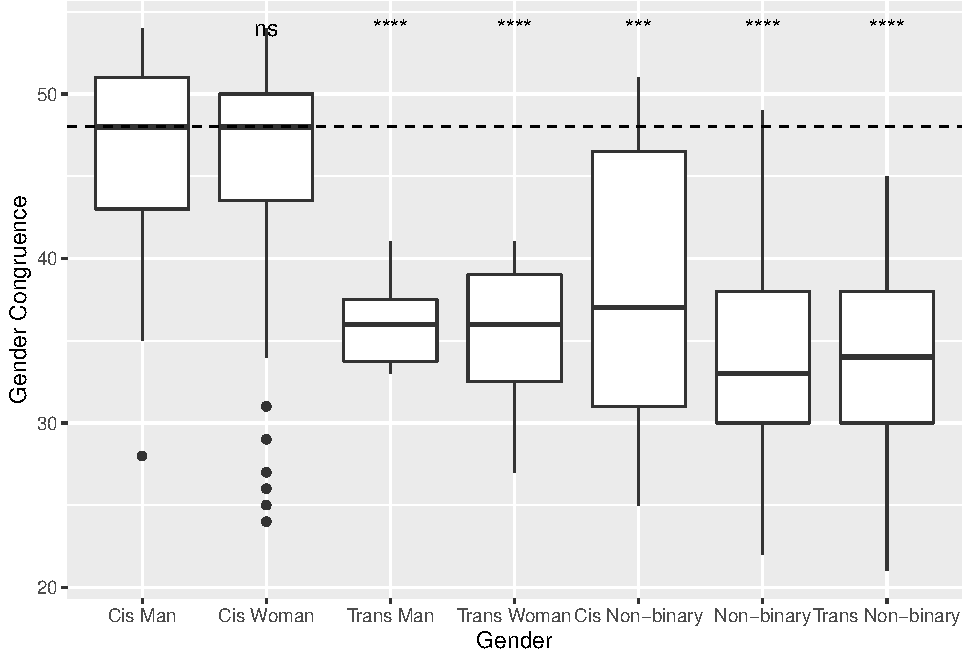
\includegraphics{thesis_files/figure-latex/unnamed-chunk-7-1.pdf}
\caption{\label{fig:unnamed-chunk-7}TCS Scores by Gender}
\end{figure}
A possible relationship between congruence and misgendering frequency was explored. A factorial ANOVA revealed that congruence had a significant effect on misgendering frequency, \emph{F}(1, 424) = 136.56, \emph{p} \textless{} 0.001 and felt stigma when misgendered, \emph{F}(1, 424) = 69.06, \emph{p} \textless{} 0.001, but not frequency and stigma when combined as a single factor, \emph{F}(1, 424) = 0.2, \emph{p} = 0.65.

\hypertarget{transgender-inclusive-behaviors}{%
\section{Transgender Inclusive Behaviors}\label{transgender-inclusive-behaviors}}

Kattari et al. (2018) developed the Transgender Inclusive Behavior Scale (TIBS) as a method of quantifying the number of behaviors that may support and include transgender people that one regularly does. Scores are a sum of responses on a series of five-point likert scales ranging from ``Never'' to ``Often.''

An independent samples t-test revealed that non-cisgender people (\emph{M} = 51.34, \emph{SD} = 9.14) reported performing more inclusive behaviors than cisgender people (\emph{M} = 41.98, \emph{SD} = 9.26), \emph{t}(304) = 10.22, \emph{p} \textless{} 0.001.

A one-way ANOVA demonstrated that there was a significant effect of gender \emph{F}(6, 260) = 26.14, \emph{p} \textless{} 0.001.
A Tukey post-hoc comparison revealed that cisgender men (\emph{M} = 37.31, \emph{SD} = 8.92) do significantly fewer trans inclusive behaviors than cisgender women (\emph{M} = 44.43, \emph{SD} = 8.18), transgender men (\emph{M} = 55.91, \emph{SD} = 9.16), transgender women (\emph{M} = 50.58, \emph{SD} = 9.97), cisgender non-binary people (\emph{M} = 45.73, \emph{SD} = 8.18), non-binary people (\emph{M} = 49.26, \emph{SD} = 9.3), and transgender non-binary people (\emph{M} = 53.85, \emph{SD} = 7.71). Cisgender women do significantly fewer trans inclusive behaviors than transgender men, transgender women, non-binary people, and transgender non-binary people. Cisgender non-binary people also do fewer trans inclusive behaviors than transgender non-binary people.
\begin{figure}
\centering
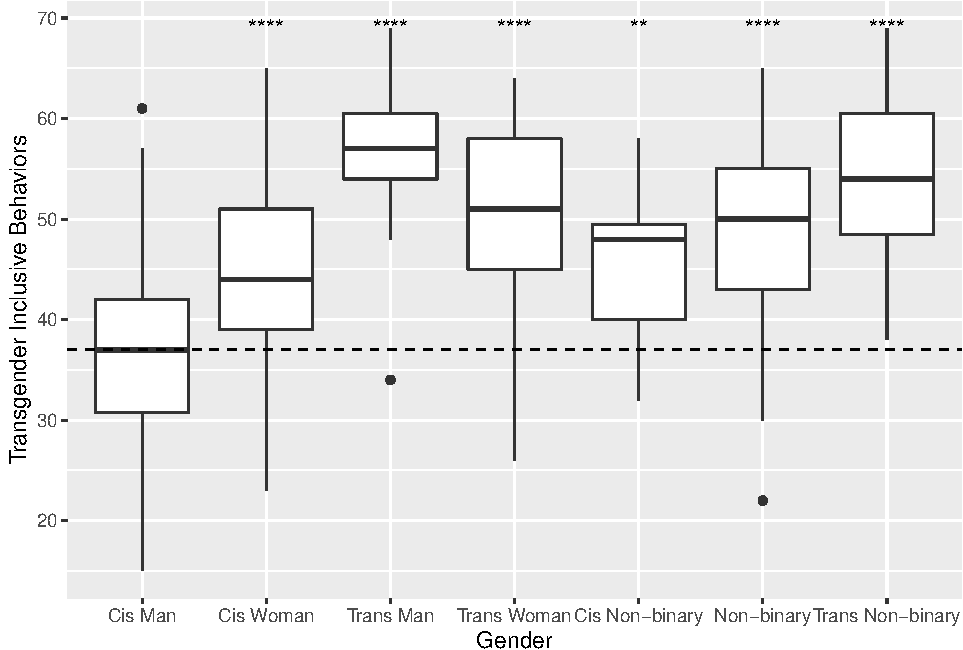
\includegraphics{thesis_files/figure-latex/unnamed-chunk-8-1.pdf}
\caption{\label{fig:unnamed-chunk-8}TIBS Scores by Gender}
\end{figure}
\hypertarget{pronouns-1}{%
\section{Pronouns}\label{pronouns-1}}

\hypertarget{comfort-sharing-pronouns}{%
\subsection{Comfort sharing pronouns}\label{comfort-sharing-pronouns}}

Items 1 (``I feel comfortable sharing my pronouns in most settings''), 2 (``I feel comfortable sharing my pronouns in non-academic settings in the Reed community''), 3 (``I feel comfortable sharing my pronouns in classes at Reed''), 7 (``I feel more comfortable sharing my pronouns if I am with people who may have similar gender identities to me''), 8 (``I feel more comfortable introducing myself with my pronouns if someone else does first''), and 9 (``I feel more comfortable introducing myself with my pronouns in class if the professor does first'') touched on participant's comfort sharing their pronouns.
A one-way ANOVA found a significant effect of setting, \emph{F}(2, 1311) = 16.39, \emph{p} \textless{} 0.001, gender, \emph{F}(6, 1311) = 40.08, \emph{p} \textless{} 0.001, and pronouns, \emph{F}(6, 1311) = 19.19, \emph{p} \textless{} 0.001, on comfort sharing pronouns. A post-hoc Tukey test found that generally, students are more comfortable sharing pronouns in class, (\emph{M} = 4.5, \emph{SD} = 0.98), and in non-academic settings at Reed, (\emph{M} = 4.43, \emph{SD} = 1.07), than they are in general, (\emph{M} = 4.14, \emph{SD} = 1.31). It also found that cisgender men, (\emph{M} = 4.65, \emph{SD} = 0.78), are more comfortable sharing their pronouns than trans men, (\emph{M} = 4.11, \emph{SD} = 1.24), trans women, (\emph{M} = 3.22, \emph{SD} = 1.51), and non-binary people, (\emph{M} = 3.66, \emph{SD} = 1.4).

One-way ANOVAs were used on each setting to elucidate effects of gender and pronoun within each setting. There were significant effects of gender in general, \emph{F}(6, 435) = 34.7, \emph{p} \textless{} 0.001, in non-academic settings at Reed, \emph{F}(6, 435) = 9.07, \emph{p} \textless{} 0.001, and in class, \emph{F}(6, 435) = 19.93, \emph{p} \textless{} 0.001. There were also significant effects of pronouns in general, \emph{F}(6, 435) = 34.7, \emph{p} \textless{} 0.001, in non-academic settings at Reed, \emph{F}(6, 435) = 9.07, \emph{p} \textless{} 0.001, and in class, \emph{F}(6, 435) = 19.93, \emph{p} \textless{} 0.001.
\begin{figure}
\centering
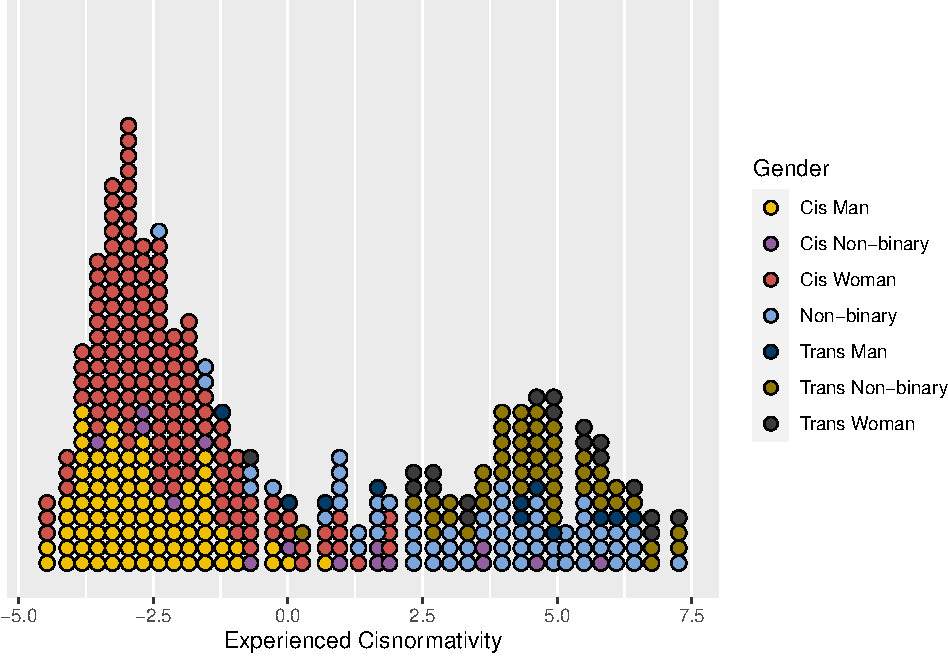
\includegraphics{thesis_files/figure-latex/unnamed-chunk-9-1.pdf}
\caption{\label{fig:unnamed-chunk-9}Responses to items 1 (``I feel comfortable sharing my pronouns in most settings''), 2 (``I feel comfortable sharing my pronouns in non-academic settings in the Reed community''), 3 (``I feel comfortable sharing my pronouns in classes at Reed'')}
\end{figure}
Post-hoc Tukey tests were used to compare gender groups within each setting. In a general setting, cis men, (\emph{M} = 4.53, \emph{SD} = 0.93), were more comfortable sharing their pronouns than trans women, (\emph{M} = 4.76, \emph{SD} = 0.68), non-binary people, (\emph{M} = 3.02, \emph{SD} = 1.5), and transgender non-binary people, (\emph{M} = 3.25, \emph{SD} = 1.49). In addition, cis women, (\emph{M} = 4.76, \emph{SD} = 0.68) were more comfortable sharing their pronouns than trans men, (\emph{M} = 3.67, \emph{SD} = 1.67), trans women, cisgender non-binary people, (\emph{M} = 3.87, \emph{SD} = 1.13), non-binary people, and transgender non-binary people. In non-academic settings at Reed, cis men, (\emph{M} = 4.59, \emph{SD} = 0.85), and cis women, (\emph{M} = 4.59, \emph{SD} = 0.85), were more comfortable sharing their pronouns than trans women, (\emph{M} = 3.4, \emph{SD} = 1.6), cis non-binary people, (\emph{M} = 3.8, \emph{SD} = 1.52), non-binary people, (\emph{M} = 4.04, \emph{SD} = 1.16), and trans non-binary people, (\emph{M} = 4.1, \emph{SD} = 1.39). In class, cis men, (\emph{M} = 4.74, \emph{SD} = 0.6), and cis women, (\emph{M} = 4.85, \emph{SD} = 0.53), were more comfortable sharing their pronouns than trans women, (\emph{M} = 3.35, \emph{SD} = 1.57), non-binary people, (\emph{M} = 3.82, \emph{SD} = 1.28), and trans non-binary people, (\emph{M} = 4.17, \emph{SD} = 1.14). Cis women were also more comfortable sharing their pronouns than cis non-binary people, (\emph{M} = 4.4, \emph{SD} = 0.83). Finally, trans women were less comfortable sharing their pronouns than cis non-binary people and trans non-binary people.

A one-way ANOVA was used to examine effects of social factors, gender, and pronouns on comfort sharing pronouns. Specifically, we examined whether people were more comfortable sharing their pronouns when a professor did so first, when someone else did first, and when the participant was with people of similar genders to their own. There were significant effects of social factor, \emph{F}(2, 1311) = 60.03, \emph{p} \textless{} 0.001, gender, \emph{F}(6, 1311) = 6.95, \emph{p} \textless{} 0.001, and pronouns, \emph{F}(6, 1311) = 15.66, \emph{p} \textless{} 0.001. A post-hoc Tukey test revealed that someone else saying their pronouns first makes the largest difference in making others comfortable sharing their pronouns. This is followed by the professor sharing their pronouns first, and finally the presence of people of similar genders to one's own.
\begin{figure}
\centering
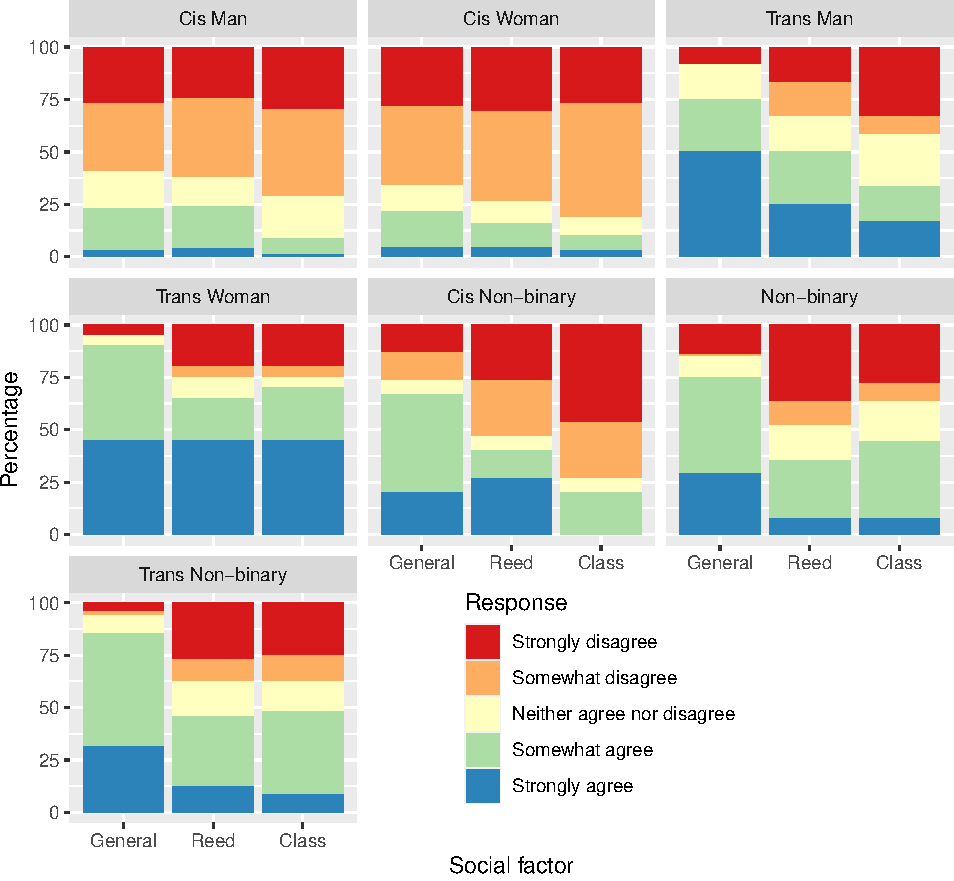
\includegraphics{thesis_files/figure-latex/unnamed-chunk-10-1.pdf}
\caption{\label{fig:unnamed-chunk-10}Responses to items 7 (``I feel more comfortable sharing my pronouns if I am with people who may have similar gender identities to me''), 8 (``I feel more comfortable introducing myself with my pronouns if someone else does first''), and 9 (``I feel more comfortable introducing myself with my pronouns in class if the professor does first'')}
\end{figure}
\hypertarget{desire-to-share-pronouns}{%
\subsection{Desire to share pronouns}\label{desire-to-share-pronouns}}

Items 4 (``I want to share my pronouns in most settings''), 5 (``I want to share my pronouns in non- academic settings in the Reed community''), and 6 (``I want to share my pronouns in classes at Reed'') touched on participant's desire to share their pronouns. A one-way ANOVA revealed significant effects of setting, \emph{F}(2, 1314) = 18.12, \emph{p} \textless{} 0.001, gender, \emph{F}(6, 1314) = 7.22, \emph{p} \textless{} 0.001, and pronouns \emph{F}(6, 1314) = 13.46, \emph{p} \textless{} 0.001. A post-hoc Tukey test revealed that people's desire to share their pronouns is highest in classroom settings, followed by non-academic settings at Reed, and then lowest in general. Trans men reported a higher desire to share their pronouns than cisgender men, cisgender women, transgender women, cisgender non-binary people, and non-binary people. Transgender non-binary people also reported a higher desire to share their pronouns than cisgender men and non-binary people.
\begin{figure}
\centering
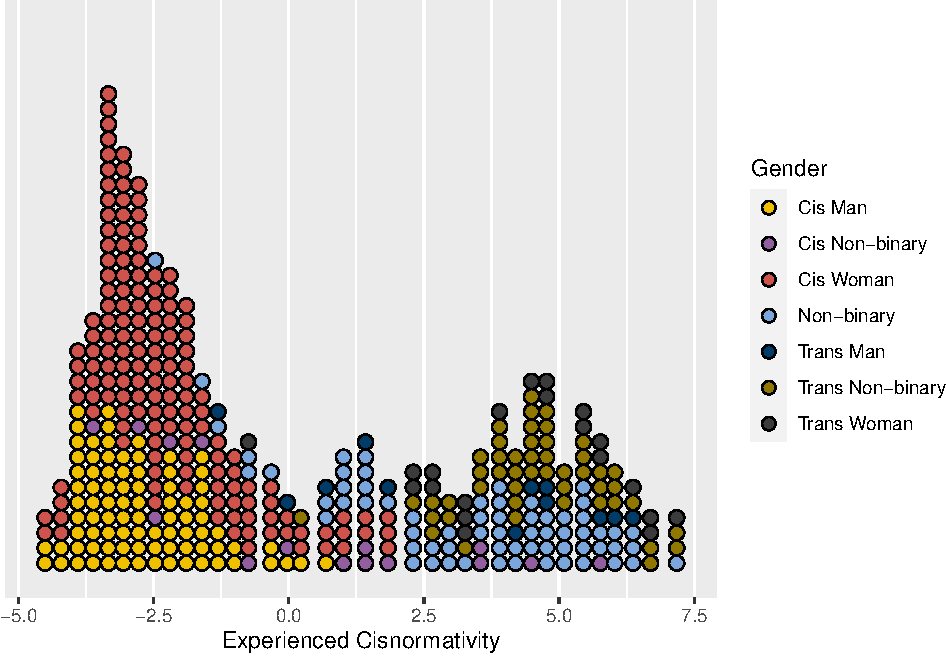
\includegraphics{thesis_files/figure-latex/unnamed-chunk-11-1.pdf}
\caption{\label{fig:unnamed-chunk-11}Responses to items 4 (``I want to share my pronouns in most settings''), 5 (``I want to share my pronouns in non- academic settings in the Reed community''), and 6 (``I want to share my pronouns in classes at Reed'')}
\end{figure}
\hypertarget{concerns-about-sharing-pronouns}{%
\subsection{Concerns about sharing pronouns}\label{concerns-about-sharing-pronouns}}

Items 10 (``I am concerned that sharing my pronouns will draw unwanted attention to myself in most settings''), 11 (``I am concerned that sharing my pronouns will draw unwanted attention to myself in non-academic settings in the Reed community''), and 12 (``I am concerned that sharing my pronouns will draw unwanted attention to myself in class at Reed'') touched on participant's concern that sharing their pronouns would draw unwanted attention to themselves. There were significant effects of setting, \emph{F}(2, 1314) = 27.49, \emph{p} \textless{} 0.001, gender \emph{F}(6, 1314) = 19.69, \emph{p} \textless{} 0.001, and pronouns, \emph{F}(6, 1314) = 23.44, \emph{p} \textless{} 0.001 on concern that sharing one's pronouns would draw unwanted attention to oneself. A post-hoc Tukey test revealed that participants were most concerned that sharing their pronouns would draw unwanted attention to them in general, followed by in non-academic settings at Reed, and least concerned in class.
\begin{figure}
\centering
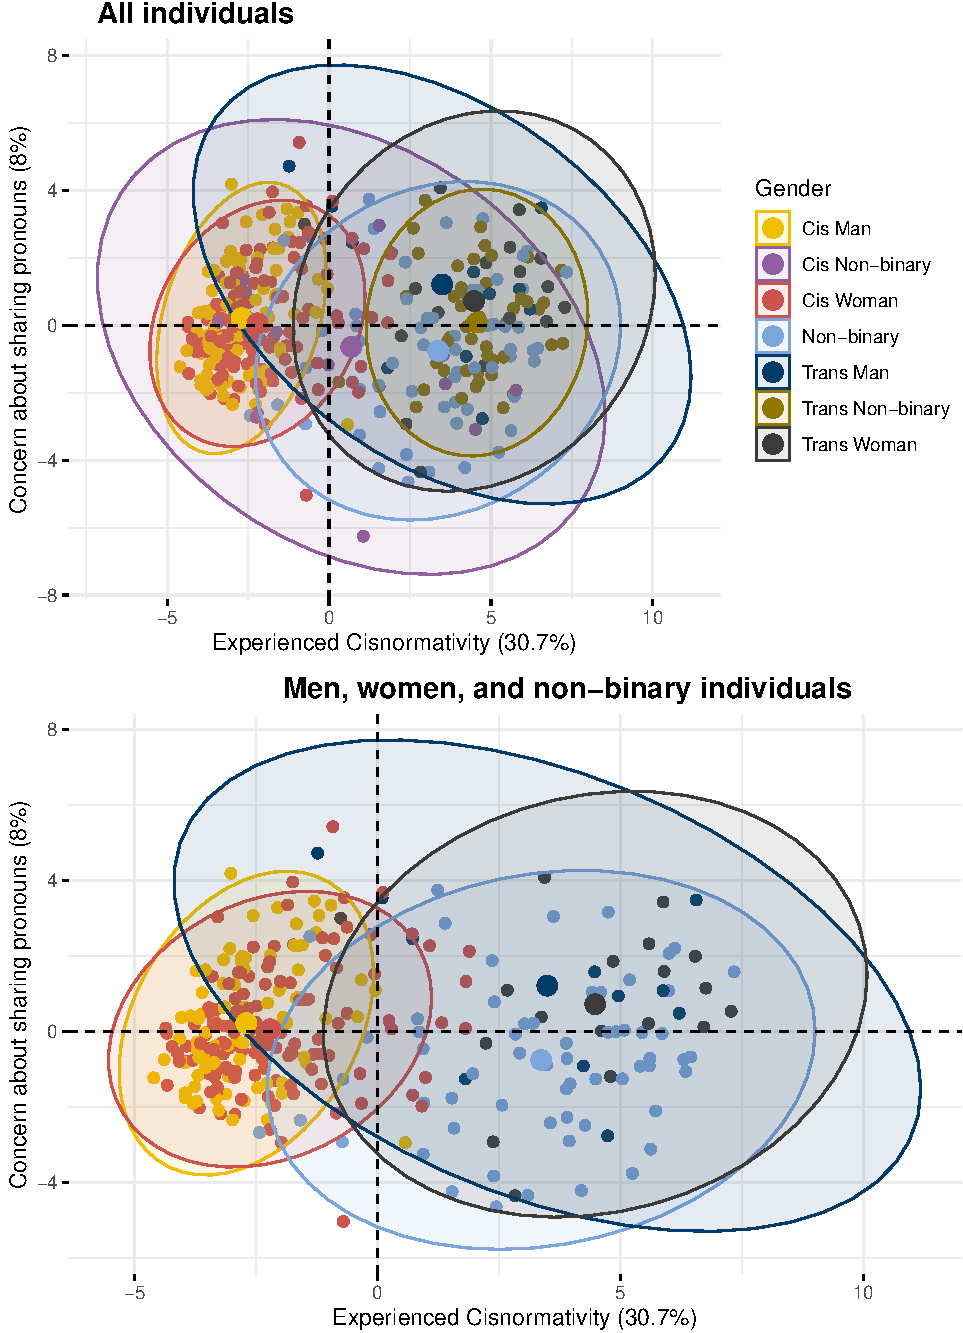
\includegraphics{thesis_files/figure-latex/unnamed-chunk-12-1.pdf}
\caption{\label{fig:unnamed-chunk-12}Responses to items 10 (``I am concerned that sharing my pronouns will draw unwanted attention to myself in most settings''), 11 (``I am concerned that sharing my pronouns will draw unwanted attention to myself in non-academic settings in the Reed community''), and 12 (``I am concerned that sharing my pronouns will draw unwanted attention to myself in class at Reed'')}
\end{figure}
\hypertarget{congruence-and-perception-of-pronouns}{%
\subsection{Congruence and perception of pronouns}\label{congruence-and-perception-of-pronouns}}

Items 13, 14, 15, 16, 17 and 18 were centered around participant's feelings of congruence between their pronouns and other aspects of their gender. We ran one-way ANOVAs examining effects of gender and pronouns on each item with post-hoc Tukey tests where relevant.

On item 13 (``I feel that the gender that people perceive me as and my pronouns are consistent with one another.''), there was a significant effect of gender, \emph{F}(6, 449) = 116.89, \emph{p} \textless{} 0.001. A post-hoc Tukey test found that cis men, (\emph{M} = 4.76, \emph{SD} = 0.6), experience higher consistency than trans men, (\emph{M} = 2.58, \emph{SD} = 1.62), trans women, (\emph{M} = 2.05, \emph{SD} = 1.1), cis non-binary people, (\emph{M} = 3.13, \emph{SD} = 1.77), non-binary people, (\emph{M} = 2.2, \emph{SD} = 1.27), and trans non-binary people, (\emph{M} = 1.85, \emph{SD} = 1.07). Cis women, (\emph{M} = 4.65, \emph{SD} = 0.85), also experience higher consistency than trans men, trans women, cis non-binary people, non-binary people, and trans non-binary people. Cis non-binary people also experience higher consistency than trans women. Finally, cis non-binary people experience higher consistency than non-binary people and trans non-binary people. There were no other significant differences between groups.

On item 14 (``I feel that my internal gender identity and pronouns are consistent with one another.''), there was a significant effect of gender, \emph{F}(6, 430) = 18.52, \emph{p} \textless{} 0.001 and pronouns, \emph{F}(6, 430) = 3.87, \emph{p} \textless{} 0.001. A post-hoc Tukey test found that cis men, (\emph{M} = 4.59, \emph{SD} = 0.8), and cis women, (\emph{M} = 4.53, \emph{SD} = 0.93), reported higher consistency than cis non-binary people, (\emph{M} = 3.07, \emph{SD} = 1.67), non-binary people, (\emph{M} = 3.23, \emph{SD} = 1.42), and trans non-binary people, (\emph{M} = 3.85, \emph{SD} = 1.34). Trans men, (\emph{M} = 4.5, \emph{SD} = 1.17), also reported higher consistency than cis non-binary people and non-binary people. Trans non-binary people also reported higher consistency than non-binary people. People who use they/them and she/her pronouns, (\emph{M} = 3.03, \emph{SD} = 1.53), reported higher consistency than people who just used they/them pronouns, (\emph{M} = 3.85, \emph{SD} = 1.21). There were no other significant differences between groups.

On item 15 (``I feel that my pronouns represent my gender identity well.''), there was a significant effect of gender, \emph{F}(6, 450) = 14.67, \emph{p} \textless{} 0.001. A post-hoc Tukey test revealed that cis men, (\emph{M} = 4.35, \emph{SD} = 1.06), and cis women, (\emph{M} = 4.39, \emph{SD} = 1.07), reported higher representativeness than cis non-binary people, (\emph{M} = 3.07, \emph{SD} = 1.67), non-binary people, (\emph{M} = 3.11, \emph{SD} = 1.46), and trans non-binary people, (\emph{M} = 3.71, \emph{SD} = 1.3). Furthermore, trans men, (\emph{M} = 4.5, \emph{SD} = 0.9), reported higher representativeness than cis non-binary people and non-binary people. There were no other significant differences between groups.
\begin{figure}
\centering
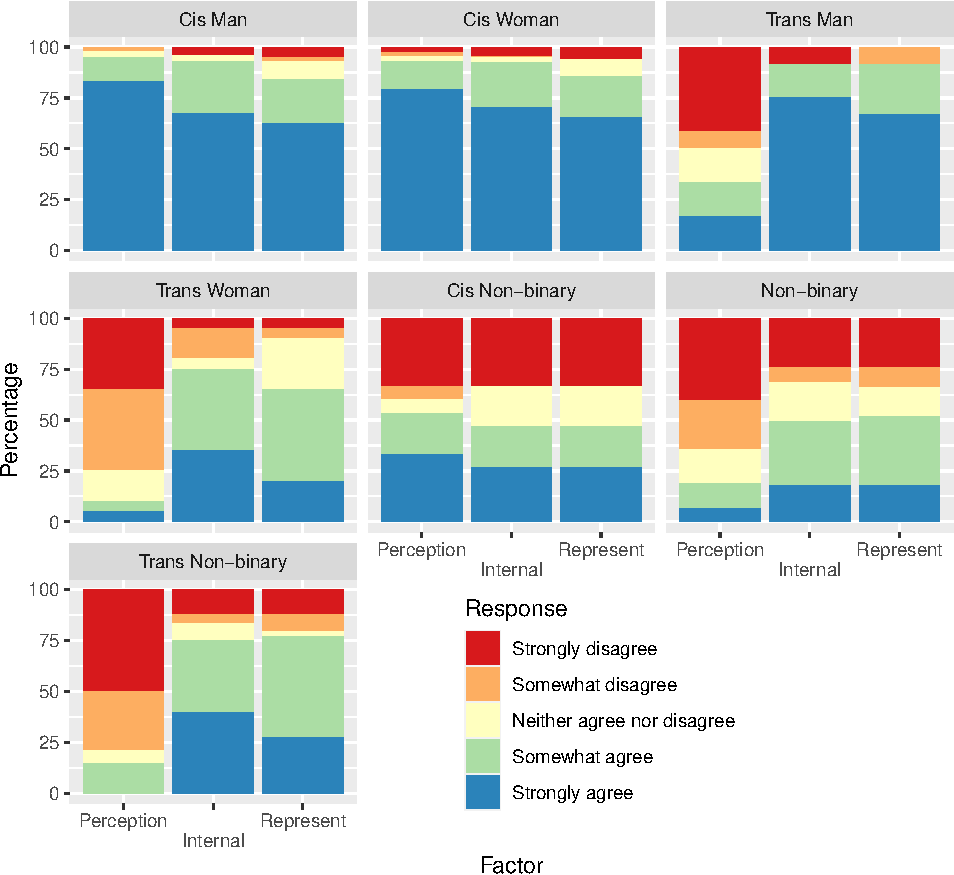
\includegraphics{thesis_files/figure-latex/unnamed-chunk-13-1.pdf}
\caption{\label{fig:unnamed-chunk-13}Responses to items 13 (``I feel that the gender that people perceive me as and my pronouns are consistent with one another.''), 14 (``I feel that my internal gender identity and pronouns are consistent with one another.''), and 15 (``I feel that my pronouns represent my gender identity well.'')}
\end{figure}
On item 16 (``If I don't tell people what my pronouns are, they will misgender me.''), there was a significant effect of gender, \emph{F}(6, 450) = 75.91, \emph{p} \textless{} 0.001. A post-hoc Tukey test revealed that cis men, (\emph{M} = 1.95, \emph{SD} = 0.3), and cis women, (\emph{M} = 1.91, \emph{SD} = 0.47), are misgendered significantly less when they do not share their pronouns when compared to trans men, (\emph{M} = 3.75, \emph{SD} = 1.54), trans women, (\emph{M} = 4.1, \emph{SD} = 1.25), non-binary people, (\emph{M} = 3.32, \emph{SD} = 1.54), and trans non-binary people, (\emph{M} = 4.31, \emph{SD} = 1.17). Furthermore, cis non-binary, (\emph{M} = 2.47, \emph{SD} = 0.92), people are misgendered significantly less than trans men, trans women, and non-binary people. There were no other significant differences between groups.

On item 17 (``I don't need to tell people what my pronouns are, because they usually assume correctly.''), there was a significant effect of gender, \emph{F}(6, 449) = 78.45, \emph{p} \textless{} 0.001. A post-hoc Tukey test revealed that people correctly assume cis men's, (\emph{M} = 4.56, \emph{SD} = 0.95), and cis women's, (\emph{M} = 4.49, \emph{SD} = 1.09), pronouns more frequently when compared to trans men, (\emph{M} = 2.5, \emph{SD} = 1.17), trans women, (\emph{M} = 2.15, \emph{SD} = 1.04), cis non-binary people, (\emph{M} = 3.27, \emph{SD} = 1.58), non-binary people, (\emph{M} = 2.46, \emph{SD} = 1.2), and trans non-binary people, (\emph{M} = 1.92, \emph{SD} = 0.65). Cis non-binary people's pronouns are also assumed correctly more frequently than trans women's and trans non-binary people.
\begin{figure}
\centering
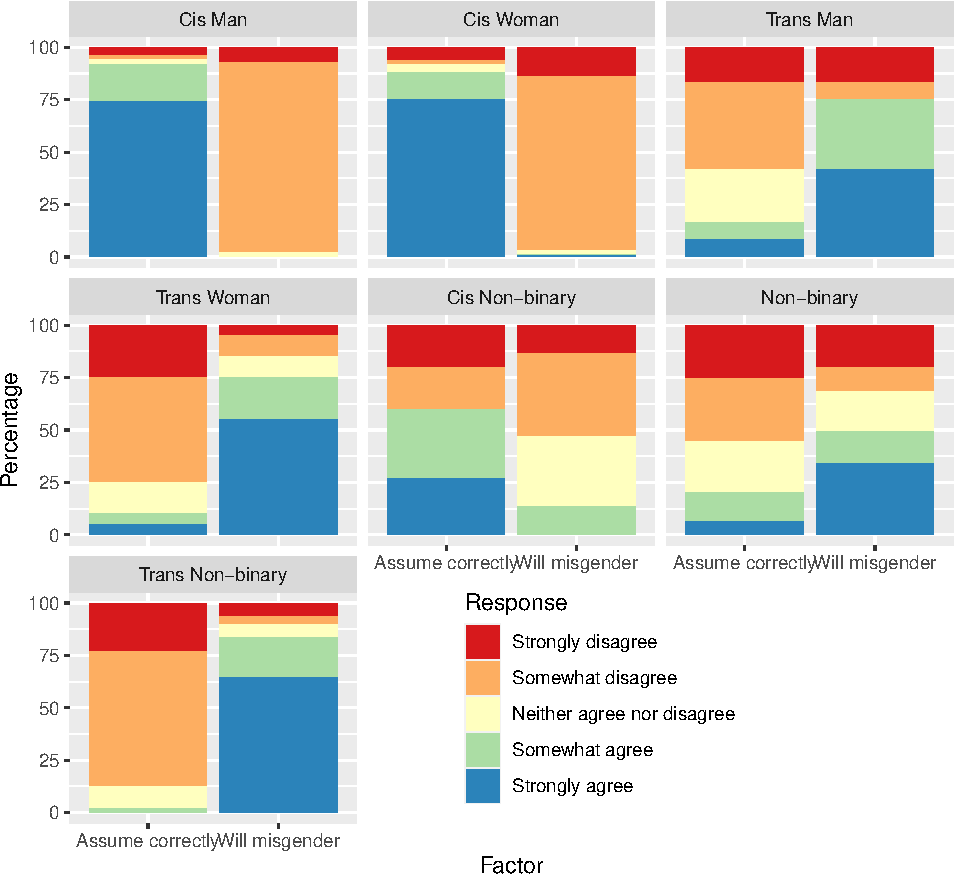
\includegraphics{thesis_files/figure-latex/unnamed-chunk-14-1.pdf}
\caption{\label{fig:unnamed-chunk-14}Responses to items 16 (``If I don't tell people what my pronouns are, they will misgender me.'') and 17 (``I don't need to tell people what my pronouns are, because they usually assume correctly.'')}
\end{figure}
Finally, on item 18 (``I feel like people understand me better when I share my pronouns.''), there was a significant effect of gender, \emph{F}(6, 449) = 25.69, \emph{p} \textless{} 0.001. A post-hoc Tukey test revealed that trans men, (\emph{M} = 3.58, \emph{SD} = 1.56), trans women, (\emph{M} = 3.7, \emph{SD} = 1.22), non-binary people, (\emph{M} = 3.67, \emph{SD} = 1.22), and trans non-binary, (\emph{M} = 3.98, \emph{SD} = 1.12), people feel better understood when they share their pronouns when compared to cis men, (\emph{M} = 2.39, \emph{SD} = 0.93) and cis women, (\emph{M} = 2.54, \emph{SD} = 0.96).
\begin{figure}
\centering
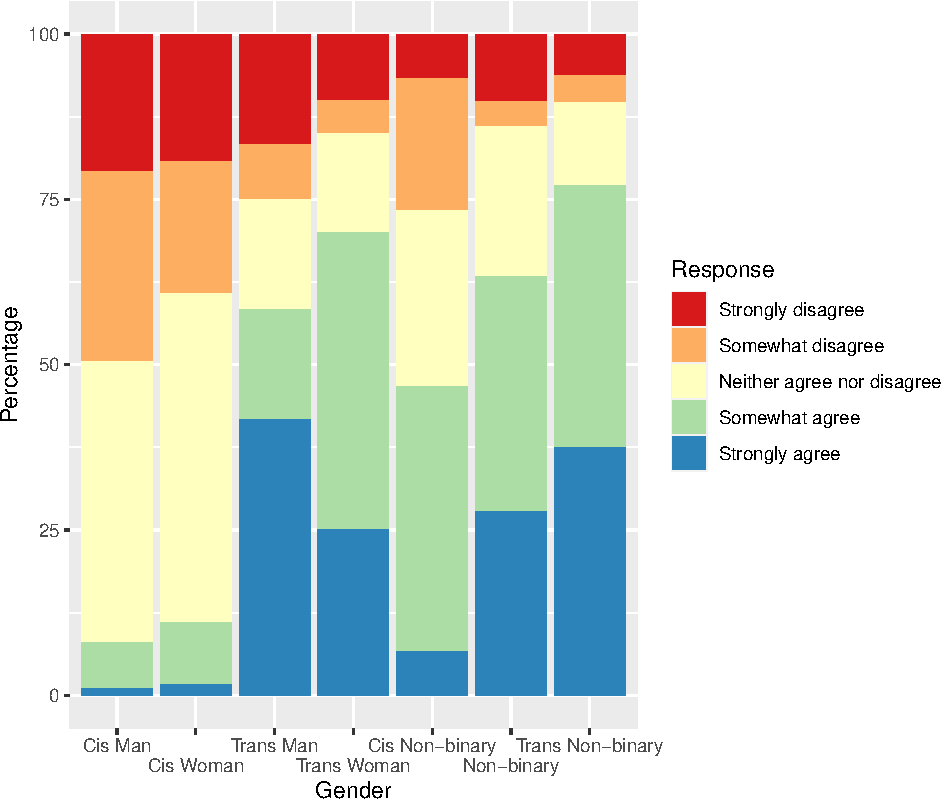
\includegraphics{thesis_files/figure-latex/unnamed-chunk-15-1.pdf}
\caption{\label{fig:unnamed-chunk-15}Responses to item 18 (``I feel like people understand me better when I share my pronouns.'')}
\end{figure}
\hypertarget{historical-experience-at-reed-college}{%
\subsection{Historical experience at Reed College}\label{historical-experience-at-reed-college}}

Item 19 (``In classes at Reed, professors usually introduce themselves with their pronouns'') asked students to report how frequently professors introduced themselves with their pronouns. A one-way ANOVA did not find a significant effect of gender, \emph{F}(6, 339) = 1.97, \emph{p} = 0.07, or major, \emph{F}(70, 339) = 1.26, \emph{p} = 0.1, on reported frequency of professors sharing their pronouns. However, when we only compared majors in which we had more than 6 students in, there was a significant effect of major, \emph{F}(18, 301) = 2.23, \emph{p} \textless{} 0.001, but not gender, \emph{F}(6, 301) = 2.04, \emph{p} = 0.06.
\begin{figure}
\centering
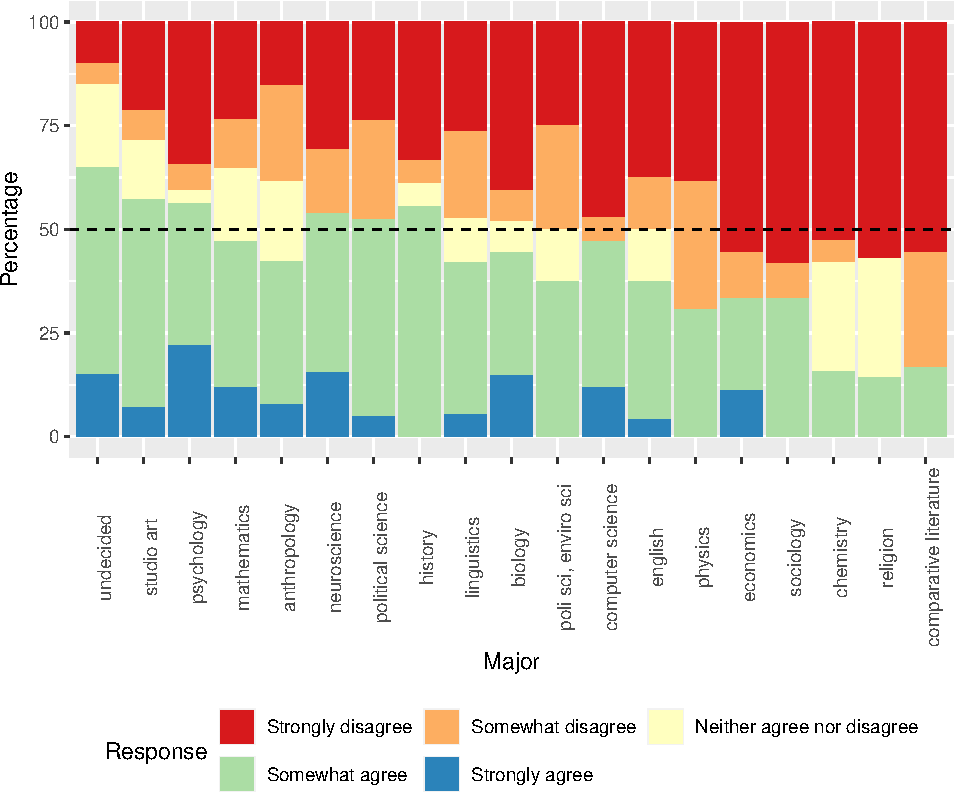
\includegraphics{thesis_files/figure-latex/unnamed-chunk-16-1.pdf}
\caption{\label{fig:unnamed-chunk-16}Responses to items 19 (``In classes at Reed, professors usually introduce themselves with their pronouns'')}
\end{figure}
Item 20 (``In classes at Reed, students usually introduce themselves with their pronouns'') asked students to report how often their peers introduced themselves with their pronouns. A one-way ANOVA revealed a significant effect of gender, \emph{F}(6, 339) = 3.67, \emph{p} \textless{} 0.001, but not major. When we only compared majors that we had more than 6 students in, there were significant effects of gender, \emph{F}(6, 301) = 3.17, \emph{p} \textless{} 0.001, but not major, \emph{F}(18, 301) = 1.35, \emph{p} = 0.16. A post-hoc Tukey test revealed that trans women, (\emph{M} = 2.25, \emph{SD} = 1), report that students share their pronouns significantly less than cis men, (\emph{M} = 2.99, \emph{SD} = 0.93), cis women, (\emph{M} = 3.12, \emph{SD} = 0.75), cis non-binary people, (\emph{M} = 3.33, \emph{SD} = 0.49), and non-binary people, (\emph{M} = 2.98, \emph{SD} = 0.81) do.
\begin{figure}
\centering
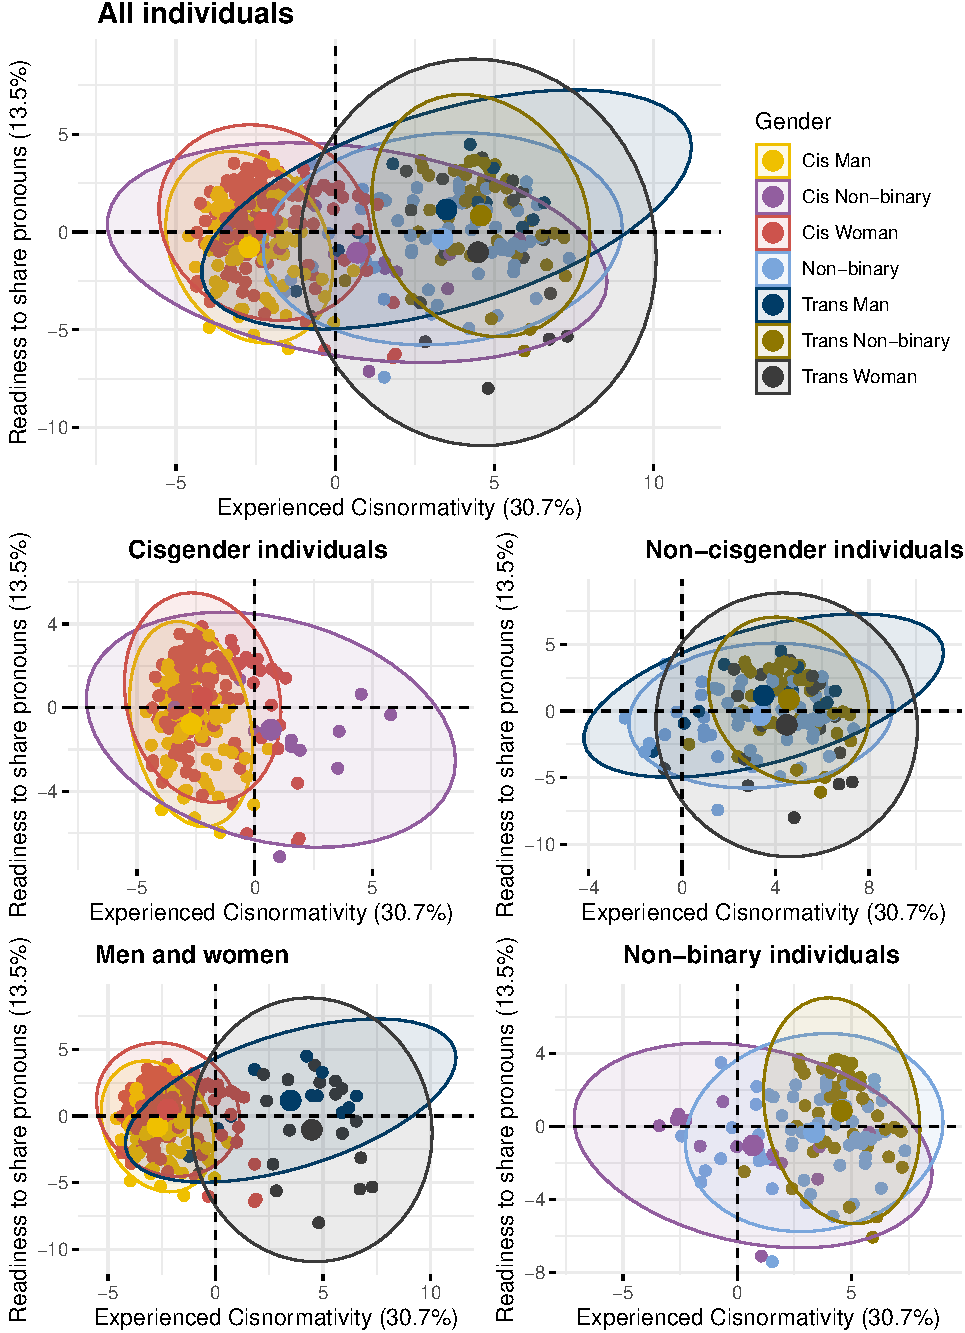
\includegraphics{thesis_files/figure-latex/unnamed-chunk-17-1.pdf}
\caption{\label{fig:unnamed-chunk-17}Responses to items 20 (``In classes at Reed, students usually introduce themselves with their pronouns'')}
\end{figure}
It should be noted that no participants responded ``Strongly disagree'' to item 20, indicating that it's common for at least some students to share their pronouns in most classes.

\hypertarget{primary-component-analysis}{%
\subsection{Primary Component Analysis}\label{primary-component-analysis}}

Principal component analysis (PCA) is a method of simplifying a model containing many variables to a small number of components that explain more variation than one component could do alone. We used PCA on the pronoun and misgendering data. Using a Screen plot, we retained three components with an eigenvalue of 3.07, accounting for 52.16\% of the variance.
\begin{longtable}[t]{lrrr}
\caption{\label{tab:unnamed-chunk-18}PCA Component Loadings. Variables are results from the survey, in order of presentation.}\\
\toprule
Variable & Comp. 1 & Comp. 2 & Comp. 3\\
\midrule
cis & -0.12 & -0.01 & 0.01\\
trans & 0.07 & 0.02 & 0.03\\
nonbinary & 0.11 & 0.01 & -0.02\\
gender.man & -0.04 & -0.03 & 0.02\\
gender.woman & -0.05 & 0.02 & 0.01\\
\addlinespace
comfort\_general & -0.26 & 0.21 & 0.09\\
comfort\_reed & -0.12 & 0.22 & 0.00\\
comfort\_class & -0.15 & 0.21 & 0.04\\
desire\_general & 0.02 & 0.42 & 0.03\\
desire\_reed & 0.11 & 0.42 & -0.04\\
\addlinespace
desire\_class & 0.06 & 0.41 & -0.03\\
comfort\_withsimilargenders & 0.27 & 0.21 & -0.03\\
comfort\_someoneelsefirst & 0.03 & 0.16 & 0.22\\
comfort\_proffirst & 0.04 & 0.18 & 0.21\\
attention\_general & 0.27 & -0.15 & 0.38\\
\addlinespace
attention\_reed & 0.12 & -0.18 & 0.56\\
attention\_class & 0.16 & -0.14 & 0.37\\
gender\_perception\_consistent & -0.40 & 0.03 & 0.26\\
gender\_pronouns\_consistent & -0.15 & 0.21 & 0.25\\
pronouns\_represent & -0.14 & 0.22 & 0.28\\
\addlinespace
willmisgender\_ifnopronouns & 0.30 & 0.09 & -0.06\\
assume\_pronouns\_correctly & -0.37 & -0.03 & 0.13\\
understand\_better & 0.20 & 0.19 & 0.03\\
profs\_share & -0.08 & 0.02 & -0.18\\
students\_share & -0.03 & 0.04 & -0.07\\
\addlinespace
reed\_support & -0.19 & -0.09 & -0.05\\
misgendering\_freq & 0.30 & 0.02 & -0.08\\
misgendering\_stigma & 0.24 & 0.12 & 0.14\\
\bottomrule
\end{longtable}
Inspection of the first component's loadings indicate that consistency between others' perception of one's gender, others' assumptions about gender and pronouns, misgendering, and comfort when with people with similar genders to one's own are making significant contributions to the first component. Because these items are mainly concerned with the assumptions other people place on one's gender and pronouns, this component appears to be the amount that cisnormative assumptions about one's gender and appearance harms individuals.

Loadings from the second component encompasses one's desire to share one's pronouns in various settings, as well as how comfortable one feels doing so. Because the largest loading in the second component is one's desire to share pronouns, this seems to indicate one's readiness to share pronouns.

Loadings from the third component emphasize concern that sharing one's pronouns will draw unwanted attention, as well as when others---not necessarily of the same gender---share their pronouns first and how consistent and representative one's pronouns are with one's gender. This component appears to represent concern around sharing pronouns and fears of judgment or lack of understanding about one's pronouns. While this may seem like the inverse of component 2, it's possible that one may not \emph{want} to share their pronouns, but be relatively unconcerned that doing so would draw unwanted attention or harm. So, we retained component 3 in addition to component 2.
\begin{figure}
\centering
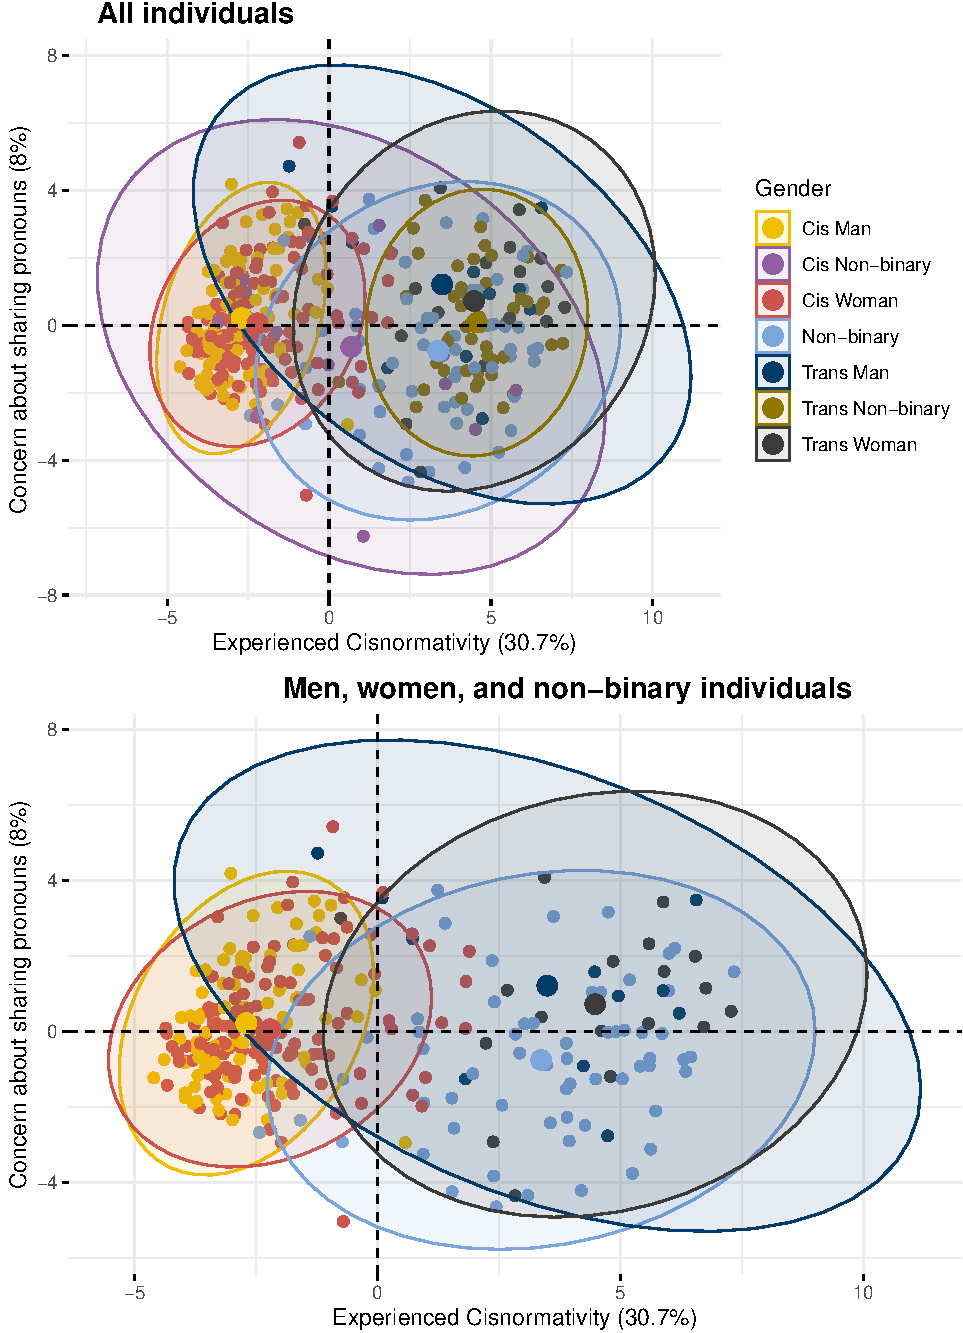
\includegraphics{thesis_files/figure-latex/unnamed-chunk-19-1.pdf}
\caption{\label{fig:unnamed-chunk-19}PCA Components 1 \& 2 by Gender. Percentage values along the axes represent \% variation in the data explained by the component.}
\end{figure}
A one-way ANOVA indicated a significant effect of gender, \emph{F}(6, 377) = 219.3, \emph{p} \textless{} 0.001 on the first component. A post-hoc Tukey test revealed that cisgender men, (\emph{M} = -2.7, \emph{SD} = 1.05), and women, (\emph{M} = -2.21, \emph{SD} = 1.35), are significantly less affected by cisnormativity than trans men, (\emph{M} = 3.49, \emph{SD} = 2.68), trans women, (\emph{M} = 4.48, \emph{SD} = 2.09), cisgender non-binary people, (\emph{M} = 0.69, \emph{SD} = 2.87), non-binary people, (\emph{M} = 3.37, \emph{SD} = 2.25), and transgender non-binary people, (\emph{M} = 4.57, \emph{SD} = 1.35). Cisgender non-binary people are also less affected than trans men, trans women, non-binary people, and transgender non-binary people. Trans non-binary people are also more affected than non-binary people. Additionally, results of Spearman correlations indicated a significant negative relationship between the first component and TCS scores, \emph{rs}(382) = -0.72, \emph{p} \textless{} 0.001, and a significant positive relationship with TIBS scores, \emph{rs}(382) = 0.51, \emph{p} \textless{} 0.001.
\begin{figure}
\centering
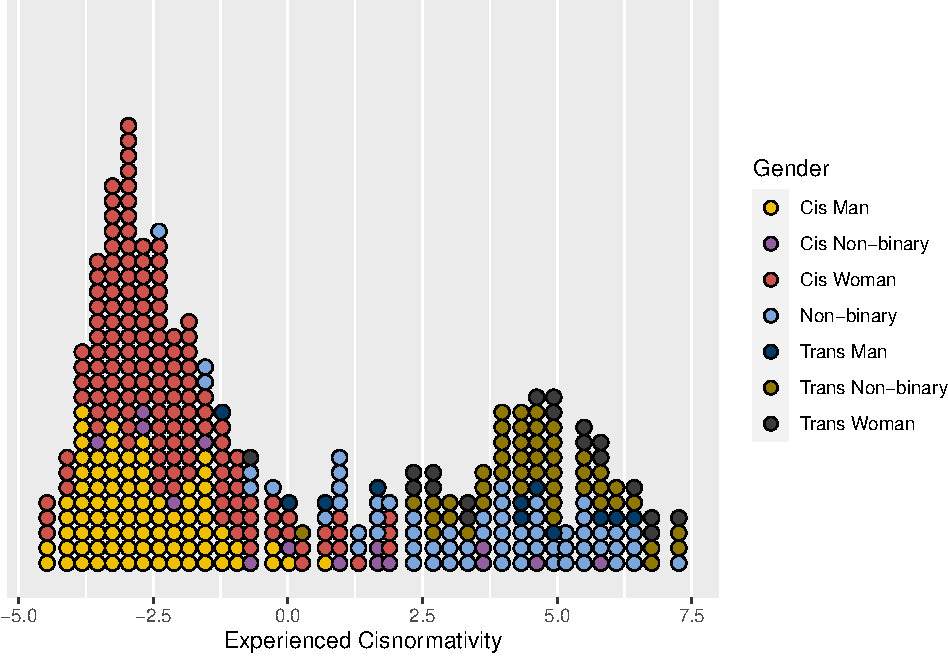
\includegraphics{thesis_files/figure-latex/unnamed-chunk-20-1.pdf}
\caption{\label{fig:unnamed-chunk-20}PCA Component 1 by Gender}
\end{figure}
Visualization of the first component indicated possible bimodality along the first component. Hartigan's dip test indicated that the distribution along the first component is unlikely to be unimodal, (\emph{D} = 0.031, \emph{p} = 0.009). Experiences with cisnormativity may be as bimodal. This indicates that cisgender and non-cisgender people may have significantly different experiences navigating the world as their gender.

Another one-way ANOVA demonstrated a significant effect of gender, \emph{F}(6, 377) = 6.14, \emph{p} \textless{} 0.001 on the second component. A post-hoc Tukey test revealed that cisgender men, (\emph{M} = -2.7, \emph{SD} = 1.05), are less willing to share their pronouns than cisgender women, (\emph{M} = -2.21, \emph{SD} = 1.35) trans men, (\emph{M} = 3.49, \emph{SD} = 2.68), and non-binary people, (\emph{M} = 3.37, \emph{SD} = 2.25). Non-binary people are also more willing to share their pronouns than transgender women, (\emph{M} = 4.48, \emph{SD} = 2.09). Additionally, results of Spearman correlations indicated a significant positive relationship between the second component, TCS scores, \emph{rs}(382) = 0.16, \emph{p} \textless{} 0.01, and TIBS scores, \emph{rs}(382) = 0.35, \emph{p} \textless{} 0.001.
\begin{figure}
\centering
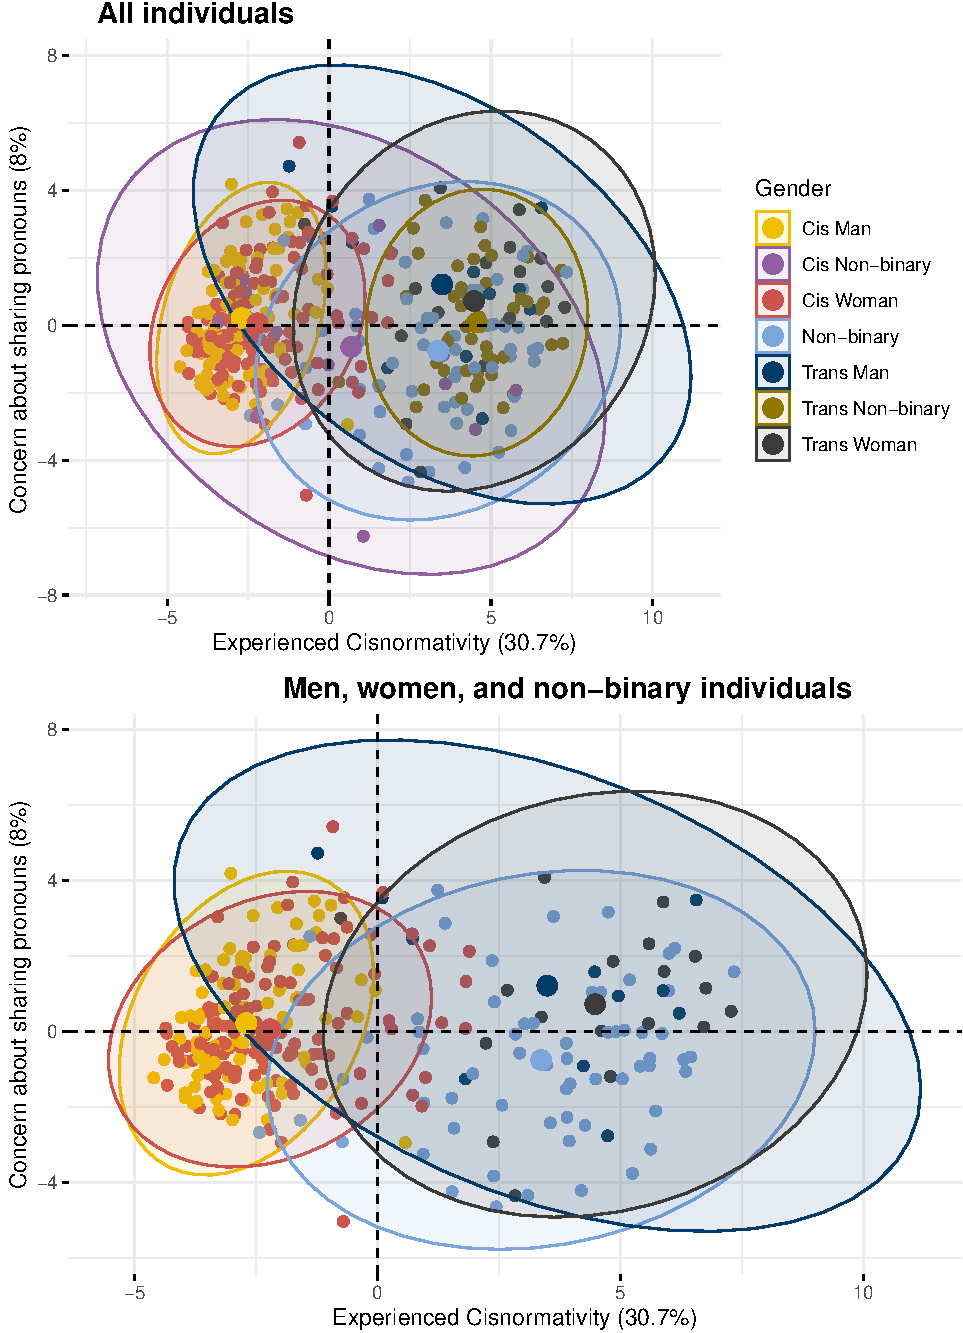
\includegraphics{thesis_files/figure-latex/unnamed-chunk-21-1.pdf}
\caption{\label{fig:unnamed-chunk-21}PCA Components 1 \& 3 by Gender. Percentage values along the axes represent \% variation in the data explained by the component.}
\end{figure}
A final one-way ANOVA demonstrated a significant effect of gender, \emph{F}(6, 377) = 4.09, \emph{p} \textless{} 0.001, TCS scores, \emph{F}(377, 377) = NA, \emph{p} \textless{} 0.001, and TIBS scores, NA, on the third component. Non-binary people, (\emph{M} = 3.37, \emph{SD} = 2.25), are significantly less concerned that sharing their pronouns will draw unwanted attention than cisgender men, (\emph{M} = -2.7, \emph{SD} = 1.05), cisgender women, (\emph{M} = -2.21, \emph{SD} = 1.35), transgender men (\emph{M} = 3.49, \emph{SD} = 2.68), and transgender women (\emph{M} = 4.48, \emph{SD} = 2.09). There were no significant effects between any other groups. Additionally, results of Spearman correlations indicated a significant positive relationship between the third component, TCS scores, \emph{rs}(382) = 0.15, \emph{p} \textless{} 0.01, and TIBS scores, \emph{rs}(382) = 0.1, \emph{p} = 0.05.

This may be due to the fact that this is the third component which only accounts for 8\% of the total variation. Visualization of the third component shows that there is considerable variation within groups. This may be due to the orthogonal nature of PCA in which it attempts to find the line that explains the greatest amount of variation, given the constraints of the previous components. Given that the first component (cisnormativity) explains the greatest amount of variation, we see less variation in concern around sharing pronouns.

\hypertarget{discussion}{%
\chapter{Discussion}\label{discussion}}

In this study, we developed and administered a number of novel items that asked participants about their relationship and feelings towards their pronouns. We also expanded gender-related demographic questions to allow for freer self-identification while retaining significant diagnostic capability. These items were administered along with questions about gender congruence and trans-inclusive behaviors.

\hypertarget{gender-identity-1}{%
\section{Gender Identity}\label{gender-identity-1}}

Gender identity is frequently assumed to be a binary or trinary, i.e.~men, women, and---perhaps---non-binary people. In the present study, we created seven artificial gender groups based on answers to a series of questions that disaggregated gender identity (e.g.~woman, agender, non-binary) and mode of relating to gender identity (e.g.~cis, trans, non-binary). These groups are artificial in the sense that they do not fully convey any one participant's gender and were formed from participants' responses to questions about whether they identified as cisgender, transgender, and non-binary, and whether they wrote that they were a man or woman in the write-in gender field.

In the present study, ``non-binary'' could refer to someone's gender, or it could be part of how they relate to their gender. There were 14 participants who indicated that they were non-binary, but did not describe their gender identity with the phrase ``non-binary.'' This includes trans men and women, agender people, genderfluid people, and people who describe their gender as, simply, ``queer.'' Within some circles of the trans community, it is understood that ``non-binary'' is an umbrella term that includes many different genders. However, in the author's experience, outside of the trans community, ``non-binary'' is commonly misunderstood as a discrete third gender. The data here indicate that this is a significant mistake, as there are numerous robust differences between the cis non-binary, non-binary, and trans non-binary groups. Even within these groups, the present methodology fails to capture many important aspects of gendered experiences.

For example, the present study intentionally did not ask participants what their sex or gender assigned at birth was. The author believes that this information is generally not as useful as many make it out to be, especially for research focused on social experiences of gender. However, this means that we were not able to make many inferences about, for example, transmisogyny, beyond comparing trans women to the other groups. Present queer discourse recognizes that, while for the purposes of third-parties, trans women and cis women are the same, trans women face unique issues such as transmisogyny---the specific fear and prejudice against trans women. Transmisogyny is a combination of misogyny and transphobia. Other transfeminine people face transmisogyny because they are perceived as trans women, but do not identify as women. Thus, transmisogyny affected/exempt have become possible categories that gendered experiences can fall in to (Holleb, 2019).

Future gender research should expand the lens of gendered experiences and gender identities beyond three genders, but should be careful to not seek out new binaries. At a minimum, gender should be collected in a write-in field, as this does not privilege certain gender identities over others. Even using the themes from a previous study as a definitive list of gender identities should be avoided. For example, no one in the present sample identified as Two-Spirit, an indigenous identity that can have tribe-specific meanings (Ristock, Zoccole, \& Passante, 2012) and---importantly---does not fit into Western gender systems. A series of checkboxes using data from the present study would fail to include Two-Spirit people.

Future gender research should also consider the implications that words such as ``transgender,'' ``genderqueer,'' and ``non-binary'' may carry. For example, while performing the analysis for the present study, the author shared some of her work. She received a number of questions about the ``cis non-binary'' category. After explaining that placement into the cis non-binary category was based off of how participants responded to questions about being cisgender and non-binary, people generally understood the role the category played. However, this made it clear to the author that ``non-binary'' is frequently considered a non-cisgender gender identity, and not as a possible way of relating to one's gender that they were assigned at birth.

Even ``non-cisgender'' is not a clear category. In order to compare our sample to McLemore (2015), we compared their data to participants who indicated that they were not cisgender. However, this was only possible because we did not have any gender-related inclusion criteria and asked participants if they were cisgender. There were multiple differences between the cis non-binary group and the rest of the participants. This begs the question: would the participants who fell into the cis non-binary group have responded if we had only sought out non-cisgender participants? Presently, the author does not think she has the right data to answer this question. Future gender-related studies should be careful about possible implications that their inclusion/exclusion criteria carry and be sensitive to local variation.

This also has broader implications for how gender identity is discussed. For example, one common phrase is ``trans and non-binary people'' (e.g.~The Trevor Project (2020)). This could potentially be interpreted as treating transgender people and non-binary people as two seperate groups. However, as we can see from the number of trans non-binary people in the sample, as well as from the diverse array of identities participants reported, the phrase does not perfectly match up to the reality of many gender identities. The author thinks that what's meant by the phrase is ``transgender and/or non-binary people'' or ``non-cisgender people,'' but this too has its flaws. ``Non-cisgender people'' then focuses the language on the existence of cis people, potentially making it counterproductive against generally showing an inclusive, trans-competent message. ``Transgender and/or non-binary people'' may come off as clunky language to people accustomed to the original phrase. The author believes that language used to communicate gender identity should not remain fixed and should strive to balance accuracy, clarity, and inclusiveness.

\hypertarget{pronouns-2}{%
\section{Pronouns}\label{pronouns-2}}

To the authors knowledge, this is the first quantitative study that has been done with an explicit focus on gendered pronouns. The data show that undergraduates at Reed College use almost every possible combination of gendered English pronouns, i.e.~every combination of ``he,'' ``she,'' and ``they.''

There was broad variation of pronoun usage within genders. By allowing participants to note their pronouns separately from their gender, we were able to get a more complete view of how pronoun usage varies across genders. While men and women \emph{mostly} used he/him and she/her pronouns respectively, there were many departures from this, including many cisgender people who exclusively use they/them pronouns, and one woman who uses he/him pronouns. Additionally, we saw non-binary people using all possible combinations of pronouns, including exclusively they/them, she/her, and he/him. While there were many unsurprising trends between gender identity and pronoun usage, there were no hard and fast rules.

Knowing an individual's gender identity or pronouns does not reveal what the other is. Especially given the limitation of three main pronouns in English, it is a fallacy to presume that everyone will be able to choose pronouns that perfectly represent their gender identity. This is supported by responses to item 14 (``I feel that my internal gender identity and pronouns are consistent with one another.''). If everyone was able to choose pronouns that perfectly represented their gender identity, we should not see significant variation between genders. However, we found significant differences between genders \emph{and} pronouns, demonstrating the inadequacy of pronouns at representing gender identity.

There was also variation in the order of the pronouns. For example, some participants who use they/them and she/her pronouns wrote ``they/she,'' and others wrote ``she/they.'' The order of pronouns was not analyzed in the present study. However, as the author has used many pronouns in her life, she knows that order may reflect any number of reasons, including preference or contextual usage. Some participants wrote at length about their complicated relationship with pronouns in the write-in field. For many people, relationships with pronouns extends beyond a simple statement of ``they/them'' or ``he/him,'' and may vary with closeness, context, or feelings.

\hypertarget{experiences-with-misgendering-1}{%
\section{Experiences with Misgendering}\label{experiences-with-misgendering-1}}

McLemore (2015) examined differences in misgendering frequency and felt stigma when misgendered in a non-cisgender population. We extended their study by administering their items to cis participants as well. We found robust differences between cis people and non-cis people in both misgendering frequency and felt stigma. This shows that trans and non-binary people have a significantly worse experience with pronouns---they get misgendered more frequently and feel more stigmatized when misgendered.

We also extended McLemore (2015) by including between-gender and between-pronoun comparisons. Interestingly, non-binary people reported feeling less stigmatized when misgendered than trans men and trans non-binary people. We found that gender congruence, as measured by the TCS, had significant effects on misgendering frequency as well as felt stigma. The author speculates that individuals who intentionally identify as transgender may care more about being gendered correctly. However, further study is needed to examine the feelings misgendering invokes.

It should also be noted that people who use only they/them pronouns reported being misgendered more than everyone else. Significant work needs to be done to normalize they/them pronouns, independent of gender presentation and appearance.

\hypertarget{gender-congruence-1}{%
\section{Gender Congruence}\label{gender-congruence-1}}

Kozee et al. (2012) developed the TCS to provide a measure of gender congruence for transgender people. However, we administered the TCS to cisgender people as well. We found that cis men and women experience significantly higher gender congruence than trans and non-binary people. While this isn't surprising, it's impressive that the results are so clear-cut.

\hypertarget{transgender-inclusive-behaviors-1}{%
\section{Transgender Inclusive Behaviors}\label{transgender-inclusive-behaviors-1}}

Kattari et al. (2018) developed the TIBS to provide a measure of how many trans-inclusive behaviors people do. The TIBS was developed for people of all genders. We found that cis men set a low bar---they perform significantly fewer trans-inclusive behaviors than every other gender group. Interestingly, cis women perform significantly more trans-inclusive behaviors than cis men. This may be due to social forces such as misogyny forcing cis women to be more aware of issues that affect trans people, or the absence of misogyny and transphobia allowing cis men to ignore issues that affect trans people.

\hypertarget{primary-component-analysis-1}{%
\section{Primary Component Analysis}\label{primary-component-analysis-1}}

Use of PCA allowed us to reduce responses to all of the pronoun-related questions to three main components. As previously discussed, the first component loadings indicated that it captured consistency between others' perception of one's gender, others' assumptions about gender and pronouns, misgendering, and comfort when with people with similar genders. Taken together, this can be interpreted to represent how strongly one is affected by cisnormativity.

Examining the variation between gender groups within the first component yields some interesting results. Firstly, as previously discussed, the distribution of individuals is likely bimodal. We can interpret this as experiences with cisnormativity falling into two groups. One could reasonably label these as cisgender and transgender. Even non-binary individuals who did not say that they were transgender fall much further to the transgender side. However, we can see from the Tukey test that they are not as affected as the trans non-binary group. These data concretely show that non-cisgender people broadly have a very different gendered experience navigating the world than cisgender people. This doesn't just manifest as different access to spaces, but as a different awareness around how their body and gender presentation is being perceived and evaluated by other people. Cis people may be entirely unaware of certain common assumptions people make about their gender and body, whereas trans and non-binary people may be acutely aware of them.

Interestingly, trans men and cis non-binary people show the greatest variation along the first component. Cisness and manhood are both systematically privileged identities that, regardless of if the individual consents to it or not, \emph{may} benefit them. Some trans men and cis non-binary people may benefit from these identities and be less affected by cisnormativiy. However, it should be noted that these two groups exhibit the greatest \emph{variation}---indicating that any given member could have a very trans or very cis experience with cisnormativity.

Loadings from the second component indicated that the component captured one's desire to share one's pronouns in various settings and well as how comfortable one feels doing so. Thus, the second component can be interpreted as one's readiness to share their pronouns.

Examining the variation between gender groups within the second component indicates that readiness to share one's pronouns may not be mediated by one single variable. It may be that cis men are uncomfortable making their gender explicit because they are frequently privileged enough to not have to think about it regularly, and so may not be as ready to share their pronouns. Trans women, on the other hand, experience lower gender congruence, and so may be more concerned that, if they say their pronouns, they will draw unwanted attention to themselves. This is reflected in the data on trans women in the third component.

The author strongly cautions against making any connection between cis men and trans women's lower readiness to share their pronouns and their gender assigned at birth---as the data show, trans women and cis men have \emph{very} different experiences in \emph{many} ways. Attempting to draw out such a conclusion is contrived at best and transphobic at worst. Furthermore, the difference between non-binary people and transgender women indicate that there is something unique about non-cisgender experiences that make trans women less ready to share their pronouns.

Loadings from the third component indicated that the component captured concern that sharing one's pronouns will draw unwanted attention, as well as when others---not necessarily of the same gender---share their pronouns first and how consistent and representative one's pronouns are with one's gender. Thus, the third component can be interpreted as concern around sharing pronouns and fears of judgment or lack of understanding about one's pronouns.

Analysis of the variance in the third component indicates that non-binary people are least concerned that sharing their pronouns will draw unwanted attention. It may be that, with the large population of non-binary students at Reed, they are less concerned that sharing their pronouns will make them stand out from everyone else. Or, it could be that non-binary people, as a product of the cisnormative society that we all live in where pronouns are often assumed from appearance, are used to sharing and correcting other people on their pronouns. After having done it countless times, non-binary people may be (sadly) habituated to misgendering and thus exhibit less concern because they expect to have to share their pronouns.

When the third component is visualized, it appears that trans men and women are slightly more concerned that sharing their pronouns will draw unwanted attention than the rest of the gender groups. This may be because trans men and women have cisnormative-ascribed standards of ``passing,'' or standards of appearance where a naive person may assume that they are cisgender. Passing is a fraught concept that is mired in Eurocentric beauty standards and a transphobic hierarchy of appearances. Yet, for trans men and women---as the author can attest---it is virtually unavoidable. Because sharing one's pronouns may make a trans person's gender more apparent and, perhaps, in contrast to their physical appearance, trans men and women may be more concerned that sharing their pronouns will draw unwanted attention because they are concerned that they may not ``pass'' to others. It should be noted that this is entirely the fault of a cisnormative society and cis people that exerts pressure on trans people to conform to certain typified appearances that may be unattainable or not desired by the trans person.

It should also be noted that, cis men, cis women, and trans non-binary people exhibit the least variation along the third component. This may be because these groups are most \emph{likely} (not guaranteed) to use a single pronoun, and so their concern around sharing their pronouns, while likely all different from each other, are more consistent when gender is controlled for (by the first component).

\hypertarget{cisgender-people}{%
\section{Cisgender People}\label{cisgender-people}}

It is important to note that cis men were frequently the exception, rather than the norm in much of the analysis. Cis men do not face misogyny (and in fact, usually perpetrate it), nor do they face transphobia, and so are uniquely positioned to ignore issues that affect women and trans people. This is reflected in the TIBS scores: every other gender group reported performing more trans-inclusive behaviors than cis men.

This is, of course, not to single out cis men. Throughout the dataset, cisgender men and women repeatedly show less worry and report being less affected by many issues that trans and non-binary people face. However, in the context of the TIBS scores, it is clear that cis men could take a \emph{much} more active role in supporting trans people. This would likely be uncomfortable for some. Cis men would have to confront the ways that they systematically benefit from and perpetuate cisnormativity. However, as the data show, trans and non-binary people are hurting daily in ways that cis people may not even be able to imagine. It is imperative that cis people confront this reality and immediately start working to support trans people.

One possible way that this could manifest would be regularly sharing pronouns. As the data show, when someone else shares their pronouns first, \emph{everyone} feels significantly more comfortable sharing their own pronouns. While the author has heard many anecdotes from people of all genders about when they do or do not feel comfortable sharing their pronouns, these data suggest that just one person sharing their pronouns makes everyone significantly more comfortable. Furthermore, the data show that people of all genders use a great variety of pronouns. From appearance alone, one cannot truly know any other person's gender or pronouns. Regularly sharing one's pronouns---especially by cis people---is an easy and concrete way to better support trans people.

\hypertarget{limitations}{%
\section{Limitations}\label{limitations}}

Due to the global pandemic that occurred in early 2020, available time for data collection and analysis was limited. However, there are several shortcomings in this study. Firstly, most of the analysis was limited to gender and pronoun effects. While important, gender identity does not exist alone. Gender identity exists in crossroads with countless other identities. Miller et al. (2019) provide an account of how queerness and disability intersect in university students. Taking their framework and extending the analysis of this data to examine intersectional effects of age, ethnicity, and major should be done to obtain a clearer picture of how Reedies experience navigating the institution as their gender.

Furthermore, to expedite analysis, gender groups were created. While this yielded some interesting and novel results, closer analysis could be done by using the many gender-related variables. For example, while we were able to compare cis and trans men, use of the gender groups prevented us from examining if manhood itself exerted any effects. While this would complicate the analysis required, we have the privilege of a large amount of very high-resolution data gender-related data. It would be a shame to not fully utilize it.

This may have also limited the possible analyses possible from analyzing the variance in the PCA components with TCS and TIBS scores. Because there were robust effects of gender group in TCS and TIBS scores, it may be that TCS and TIBS scores only served as proxies of gender group. Because there were robust gender differences in every retained PCA component, this may have been the reason we saw effects of congruence and trans-inclusive behaviors in each component as well. It may prove more useful to include individual answers to the TCS and TIBS items in the PCA model and observe how they load with the novel items we created in this study.

Additionally, it must be acknowledged that the scope of this study is limited to undergraduates from Reed College. This is a very specific population and likely does not generalize well. While this study may prove useful in guiding other research on pronouns and gives us a unique opportunity to make institution-specific recommendations, these items should be re-assessed and administered to a more diverse population in age, ethnicity, socio-economic class, and education, to name a few.

\hypertarget{conclusion}{%
\chapter{Conclusion}\label{conclusion}}

Gendered pronouns are a relatively novel area of study for transgender literature. Yet pronouns are critical to trans people's identities and used every day as they communicate and navigate the world. To the author's knowledge, there has not been any large scale quantitative studies explicitly focused on pronouns.

We found that people of all genders use virtually all combinations of common English pronouns. To the authors knowledge, specific data on pronoun usage and gender has not been collected at scale before. While there are, of course, strong trends of certain genders using certain pronouns, there was great diversity within every gender group. Furthermore, the data suggest that people of all genders have very different relationships with pronouns. Pronouns prove a poor signifier of gender, So, they should not be considered equivalent to gender. Pronouns may be better conceptualized as a way in which others can recognize and affirm one's gender.

It's likely that even in a small group of people, assuming everyone's pronouns will like lead to misgendering one or more people, making it important to share and ask for pronouns when meeting new people. As previously established, misgendering can be significantly stigmatizing and disruptive for transgender people, and so should be avoided at all costs. Furthermore, the data show that one person sharing their pronouns will likely make everyone else feel significantly more comfortable sharing their pronouns. This is an easy but concrete way that cisgender people can support trans people.

We also developed a novel way of gathering gender-related demographic data. While imperfect, the consistent pattern of difference between cis men, cis women, trans men, trans women, cis non-binary people, non-binary people, and trans non-binary people suggest that future gender research may be well served in treating cisness, transness, and non-binary identity as modes of relating to one's gender. This gives participants the opportunity to freely define their gender, while also giving researchers additional demographic data to use in analysis.

Through the use of principal component analysis, we found that there are significant differences in how cisgender and non-cisgender navigate the world in a gendered way. Non-cisgender people are significantly more affected by cisnormativity and are much more concerned that something as simple as sharing their pronouns will bring unwanted attention to themselves than cis people. The need for concrete action and support from cis people for trans people is strong.

\appendix

\hypertarget{appendix}{%
\chapter*{Appendix}\label{appendix}}
\addcontentsline{toc}{chapter}{Appendix}

Data was imported directly from Qualtrics and processed with the following code.
\begin{Shaded}
\begin{Highlighting}[]
\KeywordTok{library}\NormalTok{(tidyverse)}
\KeywordTok{library}\NormalTok{(qualtRics)}
\KeywordTok{library}\NormalTok{(rjson)}
\KeywordTok{library}\NormalTok{(here)}

\CommentTok{\# fetch survey data from qualtrics}
\NormalTok{survey\_dat \textless{}{-}}\StringTok{ }\KeywordTok{fetch\_survey}\NormalTok{(}\DataTypeTok{surveyID =} \StringTok{"XXXXXXXXX"}\NormalTok{)}
\CommentTok{\# read in themes from qualatative analysis}
\NormalTok{themes \textless{}{-}}\StringTok{ }\KeywordTok{fromJSON}\NormalTok{(}\DataTypeTok{file =} \KeywordTok{here}\NormalTok{(}\StringTok{"index"}\NormalTok{, }\StringTok{"analysis"}\NormalTok{, }\StringTok{"themes.json"}\NormalTok{))}
\NormalTok{gender\_themes \textless{}{-}}\StringTok{ }\NormalTok{themes}\OperatorTok{$}\NormalTok{gender}
\NormalTok{pronouns\_themes \textless{}{-}}\StringTok{ }\NormalTok{themes}\OperatorTok{$}\NormalTok{pronouns}
\NormalTok{sexuality\_themes \textless{}{-}}\StringTok{ }\NormalTok{themes}\OperatorTok{$}\NormalTok{sexual}

\CommentTok{\# recode likert values}
\NormalTok{recode\_likert \textless{}{-}}\StringTok{ }\ControlFlowTok{function}\NormalTok{(data) \{}
\NormalTok{  data }\OperatorTok{\%\textgreater{}\%}
\StringTok{    }\KeywordTok{mutate\_at}\NormalTok{(}\KeywordTok{vars}\NormalTok{(}\KeywordTok{starts\_with}\NormalTok{(}\KeywordTok{c}\NormalTok{(}\StringTok{"Q18"}\NormalTok{, }\StringTok{"Q11"}\NormalTok{, }\StringTok{"Q33"}\NormalTok{, }\StringTok{"Q30"}\NormalTok{))), }
              \KeywordTok{funs}\NormalTok{(}
                \KeywordTok{recode}\NormalTok{(.,}
                                 \StringTok{"Strongly agree"}\NormalTok{ =}\StringTok{ }\DecValTok{5}\NormalTok{,}
                                 \StringTok{"Somewhat agree"}\NormalTok{ =}\StringTok{ }\DecValTok{4}\NormalTok{,}
                                 \StringTok{"Neither agree nor disagree"}\NormalTok{ =}\StringTok{ }\DecValTok{3}\NormalTok{,}
                                 \StringTok{"Strongly disagree"}\NormalTok{ =}\StringTok{ }\DecValTok{2}\NormalTok{,}
                                 \StringTok{"Somewhat disagree"}\NormalTok{ =}\StringTok{ }\DecValTok{1}
\NormalTok{                       )}
\NormalTok{                  )}
\NormalTok{              ) }\OperatorTok{\%\textgreater{}\%}
\StringTok{    }\KeywordTok{mutate\_at}\NormalTok{(}\KeywordTok{vars}\NormalTok{(}\KeywordTok{starts\_with}\NormalTok{(}\KeywordTok{c}\NormalTok{(}\StringTok{"Q17"}\NormalTok{, }\StringTok{"Q14"}\NormalTok{))), }
              \KeywordTok{funs}\NormalTok{(}\KeywordTok{recode}\NormalTok{(.,}
                                 \StringTok{"Always"}\NormalTok{ =}\StringTok{ }\DecValTok{5}\NormalTok{,}
                                 \StringTok{"Often"}\NormalTok{ =}\StringTok{ }\DecValTok{4}\NormalTok{,}
                                 \StringTok{"Sometimes"}\NormalTok{ =}\StringTok{ }\DecValTok{3}\NormalTok{,}
                                 \StringTok{"Rarely"}\NormalTok{ =}\StringTok{ }\DecValTok{2}\NormalTok{,}
                                 \StringTok{"Never"}\NormalTok{ =}\StringTok{ }\DecValTok{1}
\NormalTok{                          )}
\NormalTok{                   )}
\NormalTok{              ) }\OperatorTok{\%\textgreater{}\%}
\StringTok{    }\KeywordTok{mutate\_at}\NormalTok{(}\KeywordTok{vars}\NormalTok{(}\KeywordTok{starts\_with}\NormalTok{(}\KeywordTok{c}\NormalTok{(}\StringTok{"Q16"}\NormalTok{))), }
              \KeywordTok{funs}\NormalTok{(}\KeywordTok{recode}\NormalTok{(.,}
                          \StringTok{"Very"}\NormalTok{ =}\StringTok{ }\DecValTok{5}\NormalTok{,}
                          \StringTok{"Considerably"}\NormalTok{ =}\StringTok{ }\DecValTok{4}\NormalTok{,}
                          \StringTok{"Somewhat"}\NormalTok{ =}\StringTok{ }\DecValTok{3}\NormalTok{,}
                          \StringTok{"Slightly"}\NormalTok{ =}\StringTok{ }\DecValTok{2}\NormalTok{,}
                          \StringTok{"Not at all"}\NormalTok{ =}\StringTok{ }\DecValTok{1}
\NormalTok{              )}
\NormalTok{              )}
\NormalTok{    )}
\NormalTok{\}}

\NormalTok{convert\_factors \textless{}{-}}\StringTok{ }\ControlFlowTok{function}\NormalTok{(data) \{}
\NormalTok{  data }\OperatorTok{\%\textgreater{}\%}
\StringTok{    }\KeywordTok{mutate\_at}\NormalTok{(}\KeywordTok{vars}\NormalTok{(}\KeywordTok{starts\_with}\NormalTok{(}\KeywordTok{c}\NormalTok{(}\StringTok{"Q21"}\NormalTok{, }\StringTok{"Q3"}\NormalTok{, }\StringTok{"Q2"}\NormalTok{, }\StringTok{"Q19"}\NormalTok{, }\StringTok{"Q8"}\NormalTok{, }\StringTok{"Q11"}\NormalTok{, }\StringTok{"Q33"}\NormalTok{, }\StringTok{"Q30"}\NormalTok{))), }
              \KeywordTok{funs}\NormalTok{(factor)}
\NormalTok{    ) }\OperatorTok{\%\textgreater{}\%}
\StringTok{    }\KeywordTok{mutate\_at}\NormalTok{(}\KeywordTok{vars}\NormalTok{(}\KeywordTok{starts\_with}\NormalTok{(}\KeywordTok{c}\NormalTok{(}\StringTok{"Q11"}\NormalTok{, }\StringTok{"Q33"}\NormalTok{, }\StringTok{"Q30"}\NormalTok{))), }
              \KeywordTok{funs}\NormalTok{(as.numeric)}
\NormalTok{    )}
\NormalTok{\}}

\NormalTok{rename\_data \textless{}{-}}\StringTok{ }\ControlFlowTok{function}\NormalTok{(data) \{}
\NormalTok{  data }\OperatorTok{\%\textgreater{}\%}
\StringTok{    }\KeywordTok{rename}\NormalTok{(}\DataTypeTok{timestamp =}\NormalTok{ RecordedDate) }\OperatorTok{\%\textgreater{}\%}
\StringTok{    }\KeywordTok{rename}\NormalTok{(}\DataTypeTok{age =}\NormalTok{ Q21) }\OperatorTok{\%\textgreater{}\%}
\StringTok{    }\KeywordTok{rename}\NormalTok{(}\DataTypeTok{pronouns =} \StringTok{\textasciigrave{}}\DataTypeTok{Q3 {-} Topics}\StringTok{\textasciigrave{}}\NormalTok{) }\OperatorTok{\%\textgreater{}\%}
\StringTok{    }\KeywordTok{rename}\NormalTok{(}\DataTypeTok{gender =} \StringTok{\textasciigrave{}}\DataTypeTok{Q2 {-} Topics}\StringTok{\textasciigrave{}}\NormalTok{) }\OperatorTok{\%\textgreater{}\%}
\StringTok{    }\KeywordTok{rename}\NormalTok{(}\DataTypeTok{gender\_raw =}\NormalTok{ Q2) }\OperatorTok{\%\textgreater{}\%}
\StringTok{    }\KeywordTok{rename}\NormalTok{(}\DataTypeTok{sexuality =} \StringTok{\textasciigrave{}}\DataTypeTok{Q19 {-} Topics}\StringTok{\textasciigrave{}}\NormalTok{) }\OperatorTok{\%\textgreater{}\%}
\StringTok{    }\KeywordTok{rename}\NormalTok{(}\DataTypeTok{major =} \StringTok{\textasciigrave{}}\DataTypeTok{Q8 {-} Topics}\StringTok{\textasciigrave{}}\NormalTok{) }\OperatorTok{\%\textgreater{}\%}
\StringTok{    }\KeywordTok{rename}\NormalTok{(}\DataTypeTok{year =}\NormalTok{ Q7) }\OperatorTok{\%\textgreater{}\%}
\StringTok{    }\KeywordTok{rename}\NormalTok{(}\DataTypeTok{comfort\_general =}\NormalTok{ Q11\_}\DecValTok{1}\NormalTok{) }\OperatorTok{\%\textgreater{}\%}
\StringTok{    }\KeywordTok{rename}\NormalTok{(}\DataTypeTok{comfort\_reed =}\NormalTok{ Q11\_}\DecValTok{2}\NormalTok{) }\OperatorTok{\%\textgreater{}\%}
\StringTok{    }\KeywordTok{rename}\NormalTok{(}\DataTypeTok{comfort\_class =}\NormalTok{ Q11\_}\DecValTok{3}\NormalTok{) }\OperatorTok{\%\textgreater{}\%}
\StringTok{    }\KeywordTok{rename}\NormalTok{(}\DataTypeTok{desire\_general =}\NormalTok{ Q11\_}\DecValTok{4}\NormalTok{) }\OperatorTok{\%\textgreater{}\%}
\StringTok{    }\KeywordTok{rename}\NormalTok{(}\DataTypeTok{desire\_reed =}\NormalTok{ Q11\_}\DecValTok{5}\NormalTok{) }\OperatorTok{\%\textgreater{}\%}
\StringTok{    }\KeywordTok{rename}\NormalTok{(}\DataTypeTok{desire\_class =}\NormalTok{ Q11\_}\DecValTok{6}\NormalTok{) }\OperatorTok{\%\textgreater{}\%}
\StringTok{    }\KeywordTok{rename}\NormalTok{(}\DataTypeTok{comfort\_withsimilargenders =}\NormalTok{ Q11\_}\DecValTok{7}\NormalTok{) }\OperatorTok{\%\textgreater{}\%}
\StringTok{    }\KeywordTok{rename}\NormalTok{(}\DataTypeTok{comfort\_someoneelsefirst =}\NormalTok{ Q11\_}\DecValTok{8}\NormalTok{) }\OperatorTok{\%\textgreater{}\%}
\StringTok{    }\KeywordTok{rename}\NormalTok{(}\DataTypeTok{comfort\_proffirst =}\NormalTok{ Q11\_}\DecValTok{9}\NormalTok{) }\OperatorTok{\%\textgreater{}\%}
\StringTok{    }\KeywordTok{rename}\NormalTok{(}\DataTypeTok{attention\_general =}\NormalTok{ Q33\_}\DecValTok{1}\NormalTok{) }\OperatorTok{\%\textgreater{}\%}
\StringTok{    }\KeywordTok{rename}\NormalTok{(}\DataTypeTok{attention\_reed =}\NormalTok{ Q33\_}\DecValTok{2}\NormalTok{) }\OperatorTok{\%\textgreater{}\%}
\StringTok{    }\KeywordTok{rename}\NormalTok{(}\DataTypeTok{attention\_class =}\NormalTok{ Q33\_}\DecValTok{3}\NormalTok{) }\OperatorTok{\%\textgreater{}\%}
\StringTok{    }\KeywordTok{rename}\NormalTok{(}\DataTypeTok{gender\_perception\_consistent =}\NormalTok{ Q33\_}\DecValTok{4}\NormalTok{) }\OperatorTok{\%\textgreater{}\%}
\StringTok{    }\KeywordTok{rename}\NormalTok{(}\DataTypeTok{gender\_pronouns\_consistent =}\NormalTok{ Q33\_}\DecValTok{5}\NormalTok{) }\OperatorTok{\%\textgreater{}\%}
\StringTok{    }\KeywordTok{rename}\NormalTok{(}\DataTypeTok{pronouns\_represent =}\NormalTok{ Q33\_}\DecValTok{6}\NormalTok{) }\OperatorTok{\%\textgreater{}\%}
\StringTok{    }\KeywordTok{rename}\NormalTok{(}\DataTypeTok{willmisgender\_ifnopronouns =}\NormalTok{ Q33\_}\DecValTok{7}\NormalTok{) }\OperatorTok{\%\textgreater{}\%}
\StringTok{    }\KeywordTok{rename}\NormalTok{(}\DataTypeTok{assume\_pronouns\_correctly =}\NormalTok{ Q33\_}\DecValTok{8}\NormalTok{) }\OperatorTok{\%\textgreater{}\%}
\StringTok{    }\KeywordTok{rename}\NormalTok{(}\DataTypeTok{understand\_better =}\NormalTok{ Q33\_}\DecValTok{9}\NormalTok{) }\OperatorTok{\%\textgreater{}\%}
\StringTok{    }\KeywordTok{rename}\NormalTok{(}\DataTypeTok{profs\_share =}\NormalTok{ Q30\_}\DecValTok{1}\NormalTok{) }\OperatorTok{\%\textgreater{}\%}
\StringTok{    }\KeywordTok{rename}\NormalTok{(}\DataTypeTok{students\_share =}\NormalTok{ Q30\_}\DecValTok{2}\NormalTok{) }\OperatorTok{\%\textgreater{}\%}
\StringTok{    }\KeywordTok{rename}\NormalTok{(}\DataTypeTok{reed\_support =}\NormalTok{ Q30\_}\DecValTok{3}\NormalTok{) }\OperatorTok{\%\textgreater{}\%}
\StringTok{    }\KeywordTok{rename}\NormalTok{(}\DataTypeTok{misgendering\_freq =}\NormalTok{ Q14\_}\DecValTok{1}\NormalTok{) }\OperatorTok{\%\textgreater{}\%}
\StringTok{    }\KeywordTok{rename}\NormalTok{(}\DataTypeTok{misgendering\_stigma =}\NormalTok{ Q16\_}\DecValTok{1}\NormalTok{)}
\NormalTok{\}}

\NormalTok{recode\_data  \textless{}{-}}\StringTok{ }\ControlFlowTok{function}\NormalTok{(data) \{}
\NormalTok{  data }\OperatorTok{\%\textgreater{}\%}
\StringTok{    }\CommentTok{\# paste together ethnicity labels}
\StringTok{    }\KeywordTok{mutate}\NormalTok{(}\DataTypeTok{ethnicity =} \KeywordTok{paste}\NormalTok{(Q20\_}\DecValTok{1}\NormalTok{, Q20\_}\DecValTok{2}\NormalTok{, Q20\_}\DecValTok{3}\NormalTok{, Q20\_}\DecValTok{4}\NormalTok{, Q20\_}\DecValTok{5}\NormalTok{, Q20\_}\DecValTok{6}\NormalTok{\_TEXT, }\DataTypeTok{sep =} \StringTok{", "}\NormalTok{),}
           \CommentTok{\# remove NA values}
           \DataTypeTok{ethnicity =} \KeywordTok{gsub}\NormalTok{(}\StringTok{"(NA|, NA|NA ,)"}\NormalTok{,}\StringTok{""}\NormalTok{,ethnicity),}
           \CommentTok{\# remove leading commas}
           \DataTypeTok{ethnicity =} \KeywordTok{gsub}\NormalTok{(}\StringTok{"\^{}, "}\NormalTok{,}\StringTok{""}\NormalTok{,ethnicity),}
           \CommentTok{\# recode blank rows as prefer not to say}
           \DataTypeTok{ethnicity =} \KeywordTok{gsub}\NormalTok{(}\StringTok{"\^{}$"}\NormalTok{, }\StringTok{"Prefer not to say"}\NormalTok{, ethnicity)}
\NormalTok{    ) }\OperatorTok{\%\textgreater{}\%}
\StringTok{    }\CommentTok{\# recode raw values}
\StringTok{    }\KeywordTok{mutate}\NormalTok{(}\DataTypeTok{nonbinary =} \KeywordTok{recode}\NormalTok{(Q6, }\StringTok{"Yes"}\NormalTok{ =}\StringTok{ }\OtherTok{TRUE}\NormalTok{, }\StringTok{"No"}\NormalTok{ =}\StringTok{ }\OtherTok{FALSE}\NormalTok{, }\DataTypeTok{.default =} \OtherTok{FALSE}\NormalTok{)) }\OperatorTok{\%\textgreater{}\%}
\StringTok{    }\KeywordTok{mutate}\NormalTok{(}\DataTypeTok{trans =} \KeywordTok{recode}\NormalTok{(Q5, }\StringTok{"Yes"}\NormalTok{ =}\StringTok{ }\OtherTok{TRUE}\NormalTok{, }\StringTok{"No"}\NormalTok{ =}\StringTok{ }\OtherTok{FALSE}\NormalTok{, }\DataTypeTok{.default =} \OtherTok{FALSE}\NormalTok{)) }\OperatorTok{\%\textgreater{}\%}
\StringTok{    }\KeywordTok{mutate}\NormalTok{(}\DataTypeTok{cis =} \KeywordTok{recode}\NormalTok{(Q4, }\StringTok{"Yes"}\NormalTok{ =}\StringTok{ }\OtherTok{TRUE}\NormalTok{, }\StringTok{"No"}\NormalTok{ =}\StringTok{ }\OtherTok{FALSE}\NormalTok{, }\DataTypeTok{.default =} \OtherTok{FALSE}\NormalTok{)) }\OperatorTok{\%\textgreater{}\%}
\StringTok{    }\CommentTok{\# convert to factors and add labels}
\StringTok{    }\KeywordTok{mutate}\NormalTok{(}
      \DataTypeTok{nonbinary =} \KeywordTok{factor}\NormalTok{(nonbinary),}
      \DataTypeTok{trans =} \KeywordTok{factor}\NormalTok{(trans),}
      \DataTypeTok{cis =} \KeywordTok{factor}\NormalTok{(cis)}
\NormalTok{    )}
\NormalTok{\}}

\NormalTok{calc\_scores \textless{}{-}}\StringTok{ }\ControlFlowTok{function}\NormalTok{(data) \{}
\NormalTok{  data }\OperatorTok{\%\textgreater{}\%}
\StringTok{    }\CommentTok{\# calculate congruence values}
\StringTok{    }\KeywordTok{mutate}\NormalTok{(}
      \DataTypeTok{Q18\_6 =}\NormalTok{ Q18\_}\DecValTok{6} \OperatorTok{*}\StringTok{ }\DecValTok{{-}1}\NormalTok{,}
      \DataTypeTok{Q18\_8 =}\NormalTok{ Q18\_}\DecValTok{8} \OperatorTok{*}\StringTok{ }\DecValTok{{-}1}\NormalTok{,}
      \DataTypeTok{Q18\_10 =}\NormalTok{ Q18\_}\DecValTok{10} \OperatorTok{*}\StringTok{ }\DecValTok{{-}1}\NormalTok{,}
      \DataTypeTok{congruence =} \KeywordTok{rowSums}\NormalTok{(}\KeywordTok{select}\NormalTok{(., Q18\_}\DecValTok{1}\NormalTok{, Q18\_}\DecValTok{2}\NormalTok{, Q18\_}\DecValTok{3}\NormalTok{, Q18\_}\DecValTok{4}\NormalTok{, Q18\_}\DecValTok{5}\NormalTok{, Q18\_}\DecValTok{6}\NormalTok{, Q18\_}\DecValTok{7}\NormalTok{, Q18\_}\DecValTok{8}\NormalTok{, Q18\_}\DecValTok{9}\NormalTok{, Q18\_}\DecValTok{10}\NormalTok{, Q18\_}\DecValTok{11}\NormalTok{, Q18\_}\DecValTok{12}\NormalTok{)),}
      \DataTypeTok{inclusive\_behavior =} \KeywordTok{rowSums}\NormalTok{(}\KeywordTok{select}\NormalTok{(., Q17\_}\DecValTok{1}\NormalTok{, Q17\_}\DecValTok{2}\NormalTok{, Q17\_}\DecValTok{3}\NormalTok{, Q17\_}\DecValTok{4}\NormalTok{, Q17\_}\DecValTok{5}\NormalTok{, Q17\_}\DecValTok{6}\NormalTok{, Q17\_}\DecValTok{7}\NormalTok{, Q17\_}\DecValTok{8}\NormalTok{, Q17\_}\DecValTok{9}\NormalTok{, Q17\_}\DecValTok{10}\NormalTok{, Q17\_}\DecValTok{11}\NormalTok{, Q17\_}\DecValTok{12}\NormalTok{, Q17\_}\DecValTok{13}\NormalTok{, Q17\_}\DecValTok{14}\NormalTok{))}
\NormalTok{      ) }
\NormalTok{\}}

\NormalTok{select\_cols \textless{}{-}}\StringTok{ }\ControlFlowTok{function}\NormalTok{(data) \{}
\NormalTok{  data }\OperatorTok{\%\textgreater{}\%}
\StringTok{    }\KeywordTok{select}\NormalTok{(}\KeywordTok{c}\NormalTok{(}
\NormalTok{      timestamp,}
\NormalTok{      age,}
\NormalTok{      ethnicity,}
\NormalTok{      pronouns,}
\NormalTok{      gender,}
\NormalTok{      gender\_raw,}
\NormalTok{      sexuality,}
\NormalTok{      major,}
\NormalTok{      year,}
\NormalTok{      nonbinary,}
\NormalTok{      trans,}
\NormalTok{      cis,}
\NormalTok{      congruence,}
\NormalTok{      inclusive\_behavior,}
\NormalTok{      comfort\_general,}
\NormalTok{      comfort\_reed,}
\NormalTok{      comfort\_class,}
\NormalTok{      desire\_general,}
\NormalTok{      desire\_reed,}
\NormalTok{      desire\_class,}
\NormalTok{      comfort\_withsimilargenders,}
\NormalTok{      comfort\_someoneelsefirst,}
\NormalTok{      comfort\_proffirst,}
\NormalTok{      attention\_general,}
\NormalTok{      attention\_reed,}
\NormalTok{      attention\_class,}
\NormalTok{      gender\_perception\_consistent,}
\NormalTok{      gender\_pronouns\_consistent,}
\NormalTok{      pronouns\_represent,}
\NormalTok{      willmisgender\_ifnopronouns,}
\NormalTok{      assume\_pronouns\_correctly,}
\NormalTok{      understand\_better,}
\NormalTok{      profs\_share,}
\NormalTok{      students\_share,}
\NormalTok{      reed\_support,}
\NormalTok{      misgendering\_freq,}
\NormalTok{      misgendering\_stigma}
\NormalTok{      )}
\NormalTok{    )}
\NormalTok{\}}

\CommentTok{\# if you updated the themes in qualtrics you will need to re{-}export them and run the themes.js script}
\CommentTok{\# convert qualatatively coded themes into discrete cols with boolean values}
\NormalTok{conv\_qual \textless{}{-}}\StringTok{ }\ControlFlowTok{function}\NormalTok{(theme\_input, themes, prefix) \{}
  \CommentTok{\# add word boundaries so regex doesn\textquotesingle{}t accidentally match "woman" when searching for "man" theme, etc}
\NormalTok{  regex\_themes \textless{}{-}}\StringTok{ }\NormalTok{themes }\OperatorTok{\%\textgreater{}\%}\StringTok{ }\KeywordTok{lapply}\NormalTok{(}\ControlFlowTok{function}\NormalTok{ (theme) \{ }\KeywordTok{paste}\NormalTok{(}\StringTok{"}\CharTok{\textbackslash{}\textbackslash{}}\StringTok{b"}\NormalTok{, theme, }\StringTok{"}\CharTok{\textbackslash{}\textbackslash{}}\StringTok{b"}\NormalTok{, }\DataTypeTok{sep =} \StringTok{""}\NormalTok{) \})}
  \CommentTok{\# match themes in each row}
\NormalTok{  data \textless{}{-}}\StringTok{ }\KeywordTok{do.call}\NormalTok{(rbind.data.frame,}
    \KeywordTok{lapply}\NormalTok{(theme\_input, }\ControlFlowTok{function}\NormalTok{(match\_string) \{}
      \KeywordTok{lapply}\NormalTok{(regex\_themes, }\ControlFlowTok{function}\NormalTok{(t) \{}
        \ControlFlowTok{if}\NormalTok{ (}\KeywordTok{is.na}\NormalTok{(match\_string)) \{}
          \CommentTok{\# if participant left write in blank, set all values to false}
          \KeywordTok{factor}\NormalTok{(}\OtherTok{FALSE}\NormalTok{, }\DataTypeTok{levels =} \KeywordTok{c}\NormalTok{(}\OtherTok{FALSE}\NormalTok{, }\OtherTok{TRUE}\NormalTok{))}
\NormalTok{        \} }\ControlFlowTok{else}\NormalTok{ \{}
          \CommentTok{\# otherwise, check to see if there is a match for each theme}
          \KeywordTok{factor}\NormalTok{(}\KeywordTok{str\_detect}\NormalTok{(}\KeywordTok{as.character}\NormalTok{(match\_string), t), }\DataTypeTok{levels =} \KeywordTok{c}\NormalTok{(}\OtherTok{FALSE}\NormalTok{, }\OtherTok{TRUE}\NormalTok{))}
\NormalTok{        \}}
\NormalTok{      \})}
\NormalTok{    \})}
\NormalTok{  )}
  \CommentTok{\# replace NA\textquotesingle{}s with FALSE}
\NormalTok{  data \textless{}{-}}\StringTok{ }\NormalTok{data }\OperatorTok{\%\textgreater{}\%}
\StringTok{    }\KeywordTok{replace}\NormalTok{(}\KeywordTok{is.na}\NormalTok{(data), }\OtherTok{FALSE}\NormalTok{)}
  \CommentTok{\# create colnames by prepending prefix to themes}
\NormalTok{  theme\_colnames \textless{}{-}}\StringTok{ }\NormalTok{themes }\OperatorTok{\%\textgreater{}\%}\StringTok{ }\KeywordTok{lapply}\NormalTok{(}\ControlFlowTok{function}\NormalTok{ (theme) \{ }\KeywordTok{paste}\NormalTok{(prefix, }\StringTok{"."}\NormalTok{, theme, }\DataTypeTok{sep =} \StringTok{""}\NormalTok{) \})}
  \CommentTok{\# set col names to themes}
  \KeywordTok{colnames}\NormalTok{(data) \textless{}{-}}\StringTok{ }\NormalTok{theme\_colnames}
\NormalTok{  data}
\NormalTok{\}}

\CommentTok{\# process qualatatively identified themes}
\CommentTok{\# converts string of themes eg. woman,trans,non{-}binary into bool vals in cols}
\NormalTok{process\_qual \textless{}{-}}\StringTok{ }\ControlFlowTok{function}\NormalTok{(data) \{}
\NormalTok{  gender\_data \textless{}{-}}\StringTok{ }\KeywordTok{conv\_qual}\NormalTok{(data}\OperatorTok{$}\NormalTok{gender, gender\_themes, }\DataTypeTok{prefix =} \StringTok{"gender"}\NormalTok{)}
\NormalTok{  pronouns\_data \textless{}{-}}\StringTok{ }\KeywordTok{conv\_qual}\NormalTok{(data}\OperatorTok{$}\NormalTok{pronouns, pronouns\_themes, }\DataTypeTok{prefix =} \StringTok{"pronoun"}\NormalTok{) }\OperatorTok{\%\textgreater{}\%}
\StringTok{    }\KeywordTok{rename}\NormalTok{(}\StringTok{"pronoun.he"}\NormalTok{ =}\StringTok{ \textasciigrave{}}\DataTypeTok{pronoun.he/him}\StringTok{\textasciigrave{}}\NormalTok{, }\StringTok{"pronoun.she"}\NormalTok{ =}\StringTok{ \textasciigrave{}}\DataTypeTok{pronoun.she/her}\StringTok{\textasciigrave{}}\NormalTok{, }\StringTok{"pronoun.they"}\NormalTok{ =}\StringTok{ \textasciigrave{}}\DataTypeTok{pronoun.they/them}\StringTok{\textasciigrave{}}\NormalTok{)}
\NormalTok{  sexuality\_data \textless{}{-}}\StringTok{ }\KeywordTok{conv\_qual}\NormalTok{(data}\OperatorTok{$}\NormalTok{sexuality, sexuality\_themes, }\DataTypeTok{prefix =} \StringTok{"sexuality"}\NormalTok{)}
  
\NormalTok{  data \textless{}{-}}\StringTok{ }\KeywordTok{cbind}\NormalTok{(data, gender\_data, pronouns\_data, sexuality\_data)}
\NormalTok{\}}

\NormalTok{bin\_genders \textless{}{-}}\StringTok{ }\ControlFlowTok{function}\NormalTok{(data) \{}
\NormalTok{  data }\OperatorTok{\%\textgreater{}\%}
\StringTok{    }\CommentTok{\# bin genders into cis man, cis woman, trans man, trans woman, cis }
\StringTok{    }\KeywordTok{mutate}\NormalTok{(}\DataTypeTok{gender\_bin =} \KeywordTok{factor}\NormalTok{(}\KeywordTok{case\_when}\NormalTok{(}
      \CommentTok{\# cis == TRUE \& nonbinary == FALSE \& trans == FALSE \& man == FALSE \& woman == FALSE \textasciitilde{} "Cis",}
\NormalTok{      cis }\OperatorTok{==}\StringTok{ }\OtherTok{TRUE} \OperatorTok{\&}\StringTok{ }\NormalTok{nonbinary }\OperatorTok{==}\StringTok{ }\OtherTok{FALSE} \OperatorTok{\&}\StringTok{ }\NormalTok{trans }\OperatorTok{==}\StringTok{ }\OtherTok{FALSE} \OperatorTok{\&}\StringTok{ }\NormalTok{gender.man }\OperatorTok{==}\StringTok{ }\OtherTok{TRUE} \OperatorTok{\&}\StringTok{ }\NormalTok{gender.woman }\OperatorTok{==}\StringTok{ }\OtherTok{FALSE} \OperatorTok{\textasciitilde{}}\StringTok{ "Cis Man"}\NormalTok{,}
\NormalTok{      cis }\OperatorTok{==}\StringTok{ }\OtherTok{TRUE} \OperatorTok{\&}\StringTok{ }\NormalTok{nonbinary }\OperatorTok{==}\StringTok{ }\OtherTok{FALSE} \OperatorTok{\&}\StringTok{ }\NormalTok{trans }\OperatorTok{==}\StringTok{ }\OtherTok{FALSE} \OperatorTok{\&}\StringTok{ }\NormalTok{gender.man }\OperatorTok{==}\StringTok{ }\OtherTok{FALSE} \OperatorTok{\&}\StringTok{ }\NormalTok{gender.woman }\OperatorTok{==}\StringTok{ }\OtherTok{TRUE} \OperatorTok{\textasciitilde{}}\StringTok{ "Cis Woman"}\NormalTok{,}
\NormalTok{      cis }\OperatorTok{==}\StringTok{ }\OtherTok{FALSE} \OperatorTok{\&}\StringTok{ }\NormalTok{trans }\OperatorTok{==}\StringTok{ }\OtherTok{TRUE} \OperatorTok{\&}\StringTok{ }\NormalTok{gender.man }\OperatorTok{==}\StringTok{ }\OtherTok{TRUE} \OperatorTok{\&}\StringTok{ }\NormalTok{gender.woman }\OperatorTok{==}\StringTok{ }\OtherTok{FALSE} \OperatorTok{\textasciitilde{}}\StringTok{ "Trans Man"}\NormalTok{,}
\NormalTok{      cis }\OperatorTok{==}\StringTok{ }\OtherTok{FALSE} \OperatorTok{\&}\StringTok{ }\NormalTok{trans }\OperatorTok{==}\StringTok{ }\OtherTok{TRUE} \OperatorTok{\&}\StringTok{ }\NormalTok{gender.man }\OperatorTok{==}\StringTok{ }\OtherTok{FALSE} \OperatorTok{\&}\StringTok{ }\NormalTok{gender.woman }\OperatorTok{==}\StringTok{ }\OtherTok{TRUE} \OperatorTok{\textasciitilde{}}\StringTok{ "Trans Woman"}\NormalTok{,}
\NormalTok{      cis }\OperatorTok{==}\StringTok{ }\OtherTok{TRUE} \OperatorTok{\&}\StringTok{ }\NormalTok{nonbinary }\OperatorTok{==}\StringTok{ }\OtherTok{TRUE} \OperatorTok{\&}\StringTok{ }\NormalTok{trans }\OperatorTok{==}\StringTok{ }\OtherTok{FALSE} \OperatorTok{\textasciitilde{}}\StringTok{ "Cis Non{-}binary"}\NormalTok{,}
      \CommentTok{\# non{-}binary bin includes participants who only marked non{-}binary and participants who marked none}
      \CommentTok{\# i also decided to fold non{-}binary men and non{-}binary women into the non{-}binary group since there}
      \CommentTok{\# didn\textquotesingle{}t seem to be a lot of differences (left commented tests at bottom of file)}
\NormalTok{      cis }\OperatorTok{==}\StringTok{ }\OtherTok{FALSE} \OperatorTok{\&}\StringTok{ }\NormalTok{nonbinary }\OperatorTok{==}\StringTok{ }\OtherTok{TRUE} \OperatorTok{\&}\StringTok{ }\NormalTok{trans }\OperatorTok{==}\StringTok{ }\OtherTok{FALSE} \OperatorTok{\textasciitilde{}}\StringTok{ "Non{-}binary"}\NormalTok{,}
\NormalTok{      cis }\OperatorTok{==}\StringTok{ }\OtherTok{FALSE} \OperatorTok{\&}\StringTok{ }\NormalTok{nonbinary }\OperatorTok{==}\StringTok{ }\OtherTok{FALSE} \OperatorTok{\&}\StringTok{ }\NormalTok{trans }\OperatorTok{==}\StringTok{ }\OtherTok{FALSE} \OperatorTok{\textasciitilde{}}\StringTok{ "Non{-}binary"}\NormalTok{,}
\NormalTok{      cis }\OperatorTok{==}\StringTok{ }\OtherTok{FALSE} \OperatorTok{\&}\StringTok{ }\NormalTok{nonbinary }\OperatorTok{==}\StringTok{ }\OtherTok{TRUE} \OperatorTok{\&}\StringTok{ }\NormalTok{trans }\OperatorTok{==}\StringTok{ }\OtherTok{TRUE} \OperatorTok{\&}\StringTok{ }\NormalTok{gender.man }\OperatorTok{==}\StringTok{ }\OtherTok{FALSE} \OperatorTok{\&}\StringTok{ }\NormalTok{gender.woman }\OperatorTok{==}\StringTok{ }\OtherTok{FALSE} \OperatorTok{\textasciitilde{}}\StringTok{ "Trans Non{-}binary"}\NormalTok{,}
      \CommentTok{\# cis == FALSE \& nonbinary == TRUE \& trans == FALSE \& gender.man == TRUE \& gender.woman == FALSE \textasciitilde{} "Non{-}binary Man",}
      \CommentTok{\# cis == FALSE \& nonbinary == FALSE \& trans == FALSE \& gender.man == TRUE \& gender.woman == FALSE \textasciitilde{} "Non{-}binary Man",}
      \CommentTok{\# cis == FALSE \& nonbinary == TRUE \& trans == FALSE \& gender.man == FALSE \& gender.woman == TRUE \textasciitilde{} "Non{-}binary Woman",}
      \CommentTok{\# cis == FALSE \& nonbinary == FALSE \& trans == FALSE \& gender.man == FALSE \& gender.woman == TRUE \textasciitilde{} "Non{-}binary Woman",}
      \OtherTok{TRUE} \OperatorTok{\textasciitilde{}}\StringTok{ "other"}
\NormalTok{    ), }\DataTypeTok{levels =} \KeywordTok{c}\NormalTok{(}\StringTok{"Cis Man"}\NormalTok{,}\StringTok{"Cis Woman"}\NormalTok{,}\StringTok{"Trans Man"}\NormalTok{,}\StringTok{"Trans Woman"}\NormalTok{, }\StringTok{"Cis Non{-}binary"}\NormalTok{, }\StringTok{"Non{-}binary"}\NormalTok{,}\StringTok{"Trans Non{-}binary"}\NormalTok{))) }\OperatorTok{\%\textgreater{}\%}
\StringTok{    }\KeywordTok{mutate}\NormalTok{(}\DataTypeTok{pronoun\_bin =} \KeywordTok{case\_when}\NormalTok{(}
\NormalTok{      pronoun.he }\OperatorTok{==}\StringTok{ }\OtherTok{TRUE} \OperatorTok{\&}\StringTok{ }\NormalTok{pronoun.she }\OperatorTok{==}\StringTok{ }\OtherTok{FALSE} \OperatorTok{\&}\StringTok{ }\NormalTok{pronoun.they }\OperatorTok{==}\StringTok{ }\OtherTok{FALSE} \OperatorTok{\&}\StringTok{ }\NormalTok{pronoun.all }\OperatorTok{==}\StringTok{ }\OtherTok{FALSE} \OperatorTok{\textasciitilde{}}\StringTok{ "he/him"}\NormalTok{,}
\NormalTok{      pronoun.he }\OperatorTok{==}\StringTok{ }\OtherTok{FALSE} \OperatorTok{\&}\StringTok{ }\NormalTok{pronoun.she }\OperatorTok{==}\StringTok{ }\OtherTok{TRUE} \OperatorTok{\&}\StringTok{ }\NormalTok{pronoun.they }\OperatorTok{==}\StringTok{ }\OtherTok{FALSE} \OperatorTok{\&}\StringTok{ }\NormalTok{pronoun.all }\OperatorTok{==}\StringTok{ }\OtherTok{FALSE} \OperatorTok{\textasciitilde{}}\StringTok{ "she/her"}\NormalTok{,}
\NormalTok{      pronoun.he }\OperatorTok{==}\StringTok{ }\OtherTok{FALSE} \OperatorTok{\&}\StringTok{ }\NormalTok{pronoun.she }\OperatorTok{==}\StringTok{ }\OtherTok{FALSE} \OperatorTok{\&}\StringTok{ }\NormalTok{pronoun.they }\OperatorTok{==}\StringTok{ }\OtherTok{TRUE} \OperatorTok{\&}\StringTok{ }\NormalTok{pronoun.all }\OperatorTok{==}\StringTok{ }\OtherTok{FALSE} \OperatorTok{\textasciitilde{}}\StringTok{ "they/them"}\NormalTok{,}
\NormalTok{      pronoun.he }\OperatorTok{==}\StringTok{ }\OtherTok{TRUE} \OperatorTok{\&}\StringTok{ }\NormalTok{pronoun.she }\OperatorTok{==}\StringTok{ }\OtherTok{FALSE} \OperatorTok{\&}\StringTok{ }\NormalTok{pronoun.they }\OperatorTok{==}\StringTok{ }\OtherTok{TRUE} \OperatorTok{\&}\StringTok{ }\NormalTok{pronoun.all }\OperatorTok{==}\StringTok{ }\OtherTok{FALSE} \OperatorTok{\textasciitilde{}}\StringTok{ "he/him \& they/them"}\NormalTok{,}
\NormalTok{      pronoun.he }\OperatorTok{==}\StringTok{ }\OtherTok{FALSE} \OperatorTok{\&}\StringTok{ }\NormalTok{pronoun.she }\OperatorTok{==}\StringTok{ }\OtherTok{TRUE} \OperatorTok{\&}\StringTok{ }\NormalTok{pronoun.they }\OperatorTok{==}\StringTok{ }\OtherTok{TRUE} \OperatorTok{\&}\StringTok{ }\NormalTok{pronoun.all }\OperatorTok{==}\StringTok{ }\OtherTok{FALSE} \OperatorTok{\textasciitilde{}}\StringTok{ "she/her \& they/them"}\NormalTok{,}
\NormalTok{      pronoun.he }\OperatorTok{==}\StringTok{ }\OtherTok{TRUE} \OperatorTok{\&}\StringTok{ }\NormalTok{pronoun.she }\OperatorTok{==}\StringTok{ }\OtherTok{TRUE} \OperatorTok{\&}\StringTok{ }\NormalTok{pronoun.they }\OperatorTok{==}\StringTok{ }\OtherTok{FALSE} \OperatorTok{\&}\StringTok{ }\NormalTok{pronoun.all }\OperatorTok{==}\StringTok{ }\OtherTok{FALSE} \OperatorTok{\textasciitilde{}}\StringTok{ "he/him \& she/her"}\NormalTok{,}
\NormalTok{      pronoun.all }\OperatorTok{==}\StringTok{ }\OtherTok{TRUE} \OperatorTok{\textasciitilde{}}\StringTok{ "all pronouns"}
\NormalTok{    ))}
\NormalTok{\}}

\NormalTok{mend\_demo \textless{}{-}}\StringTok{ }\ControlFlowTok{function}\NormalTok{(data) \{}
\NormalTok{  data }\OperatorTok{\%\textgreater{}\%}
\StringTok{    }\KeywordTok{mutate}\NormalTok{(}\DataTypeTok{Q20\_6\_TEXT =} \KeywordTok{as.character}\NormalTok{(Q20\_}\DecValTok{6}\NormalTok{\_TEXT)) }\OperatorTok{\%\textgreater{}\%}
\StringTok{    }\KeywordTok{mutate}\NormalTok{(}\DataTypeTok{ethnicity =} \KeywordTok{case\_when}\NormalTok{(}
      \KeywordTok{str\_detect}\NormalTok{(}\KeywordTok{tolower}\NormalTok{(Q20\_}\DecValTok{6}\NormalTok{\_TEXT), }\StringTok{"(hispanic|latino|latinx)"}\NormalTok{) }\OperatorTok{\textasciitilde{}}\StringTok{ "Latino"}\NormalTok{,}
      \OtherTok{TRUE} \OperatorTok{\textasciitilde{}}\StringTok{ }\NormalTok{ethnicity}
\NormalTok{    )) }\OperatorTok{\%\textgreater{}\%}
\StringTok{    }\KeywordTok{mutate}\NormalTok{(}\DataTypeTok{ethnicity =} \KeywordTok{case\_when}\NormalTok{(}
      \KeywordTok{str\_detect}\NormalTok{(ethnicity, }\StringTok{","}\NormalTok{) }\OperatorTok{\textasciitilde{}}\StringTok{ "Mixed Race or Ethnicity"}\NormalTok{,}
      \OtherTok{TRUE} \OperatorTok{\textasciitilde{}}\StringTok{ }\NormalTok{ethnicity}
\NormalTok{    ))}
\NormalTok{\}}

\NormalTok{all\_resp\_mod\_data \textless{}{-}}\StringTok{ }\NormalTok{survey\_dat }\OperatorTok{\%\textgreater{}\%}
\StringTok{  }\KeywordTok{filter}\NormalTok{(Finished }\OperatorTok{==}\StringTok{ }\OtherTok{TRUE}\NormalTok{) }\OperatorTok{\%\textgreater{}\%}
\StringTok{  }\KeywordTok{recode\_likert}\NormalTok{() }\OperatorTok{\%\textgreater{}\%}
\StringTok{  }\KeywordTok{convert\_factors}\NormalTok{() }\OperatorTok{\%\textgreater{}\%}
\StringTok{  }\KeywordTok{rename\_data}\NormalTok{() }\OperatorTok{\%\textgreater{}\%}
\StringTok{  }\KeywordTok{recode\_data}\NormalTok{() }\OperatorTok{\%\textgreater{}\%}
\StringTok{  }\KeywordTok{calc\_scores}\NormalTok{() }\OperatorTok{\%\textgreater{}\%}
\StringTok{  }\KeywordTok{mend\_demo}\NormalTok{()  }\OperatorTok{\%\textgreater{}\%}
\StringTok{  }\KeywordTok{select\_cols}\NormalTok{() }\OperatorTok{\%\textgreater{}\%}
\StringTok{  }\KeywordTok{process\_qual}\NormalTok{() }\OperatorTok{\%\textgreater{}\%}
\StringTok{  }\KeywordTok{bin\_genders}\NormalTok{()}

\NormalTok{mod\_data \textless{}{-}}\StringTok{ }\NormalTok{all\_resp\_mod\_data }\OperatorTok{\%\textgreater{}\%}
\StringTok{  }\KeywordTok{filter}\NormalTok{(year }\OperatorTok{!=}\StringTok{ "Other"}\NormalTok{) }\OperatorTok{\%\textgreater{}\%}
\StringTok{  }\KeywordTok{arrange}\NormalTok{(timestamp)}

\NormalTok{total\_responses \textless{}{-}}\StringTok{ }\NormalTok{survey\_dat }\OperatorTok{\%\textgreater{}\%}
\StringTok{  }\KeywordTok{nrow}\NormalTok{()}

\NormalTok{total\_complete\_responses \textless{}{-}}\StringTok{ }\NormalTok{survey\_dat }\OperatorTok{\%\textgreater{}\%}
\StringTok{  }\KeywordTok{filter}\NormalTok{(Finished }\OperatorTok{==}\StringTok{ }\OtherTok{TRUE}\NormalTok{) }\OperatorTok{\%\textgreater{}\%}
\StringTok{  }\KeywordTok{nrow}\NormalTok{()}

\NormalTok{total\_nonundergrad \textless{}{-}}\StringTok{ }\NormalTok{all\_resp\_mod\_data }\OperatorTok{\%\textgreater{}\%}
\StringTok{  }\KeywordTok{filter}\NormalTok{(year }\OperatorTok{==}\StringTok{ "Other"}\NormalTok{) }\OperatorTok{\%\textgreater{}\%}
\StringTok{  }\KeywordTok{nrow}\NormalTok{()}
\end{Highlighting}
\end{Shaded}
Principal component analysis was done with the \texttt{prcomp} function. Implementation of the PCA is below.
\begin{Shaded}
\begin{Highlighting}[]
\NormalTok{pca\_all \textless{}{-}}\StringTok{ }\NormalTok{mod\_data }\OperatorTok{\%\textgreater{}\%}
\StringTok{  }\KeywordTok{select}\NormalTok{(}
\NormalTok{    cis,}
\NormalTok{    trans,}
\NormalTok{    nonbinary,}
\NormalTok{    gender.man,}
\NormalTok{    gender.woman,}
\NormalTok{    gender\_bin,}
\NormalTok{    pronoun\_bin,}
\NormalTok{    comfort\_general,}
\NormalTok{    comfort\_reed,}
\NormalTok{    comfort\_class,}
\NormalTok{    desire\_general,}
\NormalTok{    desire\_reed,}
\NormalTok{    desire\_class,}
\NormalTok{    comfort\_withsimilargenders,}
\NormalTok{    comfort\_someoneelsefirst,}
\NormalTok{    comfort\_proffirst,}
\NormalTok{    attention\_general,}
\NormalTok{    attention\_reed,}
\NormalTok{    attention\_class,}
\NormalTok{    gender\_perception\_consistent,}
\NormalTok{    gender\_pronouns\_consistent,}
\NormalTok{    pronouns\_represent,}
\NormalTok{    willmisgender\_ifnopronouns,}
\NormalTok{    assume\_pronouns\_correctly,}
\NormalTok{    understand\_better,}
\NormalTok{    profs\_share,}
\NormalTok{    students\_share,}
\NormalTok{    reed\_support,}
\NormalTok{    misgendering\_freq,}
\NormalTok{    misgendering\_stigma,}
\NormalTok{    inclusive\_behavior,}
\NormalTok{    congruence}
\NormalTok{    ) }\OperatorTok{\%\textgreater{}\%}
\StringTok{  }\KeywordTok{mutate}\NormalTok{(}\DataTypeTok{gender.man =} \KeywordTok{as.numeric}\NormalTok{(gender.man), }\DataTypeTok{gender.woman =} \KeywordTok{as.numeric}\NormalTok{(gender.woman), }\DataTypeTok{nonbinary =} \KeywordTok{as.numeric}\NormalTok{(nonbinary), }\DataTypeTok{trans =} \KeywordTok{as.numeric}\NormalTok{(trans), }\DataTypeTok{cis =} \KeywordTok{as.numeric}\NormalTok{(cis)) }\OperatorTok{\%\textgreater{}\%}
\StringTok{  }\KeywordTok{filter}\NormalTok{(}\KeywordTok{complete.cases}\NormalTok{(.))}

\CommentTok{\# don\textquotesingle{}t include these variables in the PCA model}
\NormalTok{pca\_in \textless{}{-}}\StringTok{ }\NormalTok{pca\_all }\OperatorTok{\%\textgreater{}\%}\StringTok{ }\KeywordTok{select}\NormalTok{(}\OperatorTok{{-}}\KeywordTok{c}\NormalTok{(pronoun\_bin, gender\_bin, inclusive\_behavior, congruence))}

\CommentTok{\# perform PCA}
\NormalTok{pca\_out \textless{}{-}}\StringTok{ }\NormalTok{pca\_in }\OperatorTok{\%\textgreater{}\%}
\StringTok{  }\KeywordTok{prcomp}\NormalTok{(}\DataTypeTok{scale =} \OtherTok{FALSE}\NormalTok{)}
\CommentTok{\# get factor loadings}
\NormalTok{loadings \textless{}{-}}\StringTok{ }\NormalTok{pca\_out }\OperatorTok{\%\textgreater{}\%}
\StringTok{  }\KeywordTok{tidy}\NormalTok{(}\StringTok{"rotation"}\NormalTok{) }\OperatorTok{\%\textgreater{}\%}
\StringTok{  }\KeywordTok{pivot\_wider}\NormalTok{(}\DataTypeTok{names\_from =}\NormalTok{ PC, }\DataTypeTok{values\_from =}\NormalTok{ value) }\OperatorTok{\%\textgreater{}\%}
\StringTok{  }\KeywordTok{select}\NormalTok{(column, }\StringTok{\textasciigrave{}}\DataTypeTok{1}\StringTok{\textasciigrave{}}\NormalTok{, }\StringTok{\textasciigrave{}}\DataTypeTok{2}\StringTok{\textasciigrave{}}\NormalTok{, }\StringTok{\textasciigrave{}}\DataTypeTok{3}\StringTok{\textasciigrave{}}\NormalTok{) }\OperatorTok{\%\textgreater{}\%}\StringTok{ }
\StringTok{  }\KeywordTok{mutate\_if}\NormalTok{(is.numeric, round, }\DataTypeTok{digits =} \DecValTok{2}\NormalTok{)}
\NormalTok{variance \textless{}{-}}\StringTok{ }\NormalTok{pca\_out }\OperatorTok{\%\textgreater{}\%}
\StringTok{  }\KeywordTok{tidy}\NormalTok{(}\StringTok{"pcs"}\NormalTok{)}
\NormalTok{eigenvals \textless{}{-}}\StringTok{ }\KeywordTok{get\_eigenvalue}\NormalTok{(pca\_out) }\OperatorTok{\%\textgreater{}\%}\StringTok{ }\KeywordTok{mutate\_if}\NormalTok{(is.numeric, round, }\DataTypeTok{digits =} \DecValTok{2}\NormalTok{)}
\end{Highlighting}
\end{Shaded}
\backmatter

\hypertarget{references}{%
\chapter*{References}\label{references}}
\addcontentsline{toc}{chapter}{References}

\markboth{References}{References}

\noindent

\setlength{\parindent}{-0.20in}
\setlength{\leftskip}{0.20in}
\setlength{\parskip}{8pt}

\hypertarget{refs}{}
\begin{cslreferences}
\leavevmode\hypertarget{ref-auerbachSWSPRESIDENTGender1999}{}%
Auerbach, J. D. (1999). FROM THE SWS PRESIDENT: Gender as Proxy. \emph{Gender \& Society}, \emph{13}(5), 581--583. \url{http://doi.org/10.1177/089124399013005001}

\leavevmode\hypertarget{ref-bradfordSocialPsychologicalHeterogeneity2019}{}%
Bradford, N. J., \& Catalpa, J. M. (2019). Social and psychological heterogeneity among binary transgender, non-binary transgender and cisgender individuals. \emph{Psychology \& Sexuality}, \emph{10}(1), 69--82. \url{http://doi.org/10.1080/19419899.2018.1552185}

\leavevmode\hypertarget{ref-diamondTransgenderExperienceIdentity2011}{}%
Diamond, L. M., Pardo, S. T., \& Butterworth, M. R. (2011). Transgender Experience and Identity. In S. J. Schwartz, K. Luyckx, \& V. L. Vignoles (Eds.), \emph{Handbook of Identity Theory and Research} (pp. 629--647). New York, NY: Springer New York. \url{http://doi.org/10.1007/978-1-4419-7988-9_26}

\leavevmode\hypertarget{ref-dozierBeardsBreastsBodies2005}{}%
Dozier, R. (2005). Beards, Breasts, and Bodies: Doing Sex in a Gendered World. \emph{Gender \& Society}, \emph{19}(3), 297--316. \url{http://doi.org/10.1177/0891243204272153}

\leavevmode\hypertarget{ref-ezieDeconstructingBodyTransgender2010}{}%
Ezie, C. (2010). \emph{Deconstructing the Body: Transgender and Intersex Identities \& Sex Discrimination -- The Need for a Strict Scrutiny Approach} (SSRN Scholarly Paper No. ID 1589519). Rochester, NY: Social Science Research Network. Retrieved from \url{https://papers.ssrn.com/abstract=1589519}

\leavevmode\hypertarget{ref-feinbergStoneButchBlues2015}{}%
Feinberg, L. (2015). \emph{Stone Butch Blues: 20th Anniversary Author Edition}. Self.

\leavevmode\hypertarget{ref-galupoConstantlyFlowingRiver2017}{}%
Galupo, M. P., Pulice-Farrow, L., \& Ramirez, J. L. (2017). ``Like a Constantly Flowing River'': Gender Identity Flexibility Among Nonbinary Transgender Individuals. In J. D. Sinnott (Ed.), \emph{Identity Flexibility During Adulthood: Perspectives in Adult Development} (pp. 163--177). Cham: Springer International Publishing. \url{http://doi.org/10.1007/978-3-319-55658-1_10}

\leavevmode\hypertarget{ref-hollebAZGenderSexuality2019}{}%
Holleb, M. L. E. (2019). \emph{The A-Z of Gender and Sexuality: From Ace to Ze}. Jessica Kingsley Publishers. Retrieved from \url{http://books.google.com?id=44F2DwAAQBAJ}

\leavevmode\hypertarget{ref-kattariDevelopmentValidationTransgender2018}{}%
Kattari, S. K., O'Connor, A. A., \& Kattari, L. (2018). Development and Validation of the Transgender Inclusive Behavior Scale (TIBS). \emph{Journal of Homosexuality}, \emph{65}(2), 181--196. \url{http://doi.org/10.1080/00918369.2017.1314160}

\leavevmode\hypertarget{ref-kozeeMeasuringTransgenderIndividuals2012}{}%
Kozee, H. B., Tylka, T. L., \& Bauerband, L. A. (2012). Measuring Transgender Individuals' Comfort With Gender Identity and Appearance: Development and Validation of the Transgender Congruence Scale. \emph{Psychology of Women Quarterly}, \emph{36}(2), 179--196. \url{http://doi.org/10.1177/0361684312442161}

\leavevmode\hypertarget{ref-kuperGenderIdentityDevelopment2018}{}%
Kuper, L. E., Wright, L., \& Mustanski, B. (2018). Gender identity development among transgender and gender nonconforming emerging adults: An intersectional approach. \emph{International Journal of Transgenderism}, \emph{19}(4), 436--455. \url{http://doi.org/10.1080/15532739.2018.1443869}

\leavevmode\hypertarget{ref-mcglashanUseAnyPronouns2018}{}%
McGlashan, H., \& Fitzpatrick, K. (2018). ``I use any pronouns, and I'm questioning everything else'': Transgender youth and the issue of gender pronouns. \emph{Sex Education}, \emph{18}(3), 239--252. \url{http://doi.org/10.1080/14681811.2017.1419949}

\leavevmode\hypertarget{ref-mclemoreExperiencesMisgenderingIdentity2015}{}%
McLemore, K. A. (2015). Experiences with Misgendering: Identity Misclassification of Transgender Spectrum Individuals. \emph{Self and Identity}, \emph{14}(1), 51--74. \url{http://doi.org/10.1080/15298868.2014.950691}

\leavevmode\hypertarget{ref-millerThisReallyInteresting2019}{}%
Miller, R. A., Wynn, R. D., \& Webb, K. W. (2019). 'This really interesting juggling act': How university students manage disability/queer identity disclosure and visibility. \emph{Journal of Diversity in Higher Education}, \emph{12}(4), 307--318. \url{http://doi.org/10.1037/dhe0000083}

\leavevmode\hypertarget{ref-modjSplitAttractionModel2017}{}%
Mod J. (2017). The Split Attraction Model- What is it? \emph{An Arospec and Acespec Safe Space}. https://aroacefaq.tumblr.com/post/143810110365/the-split-attraction-model-what-is-it.

\leavevmode\hypertarget{ref-nagoshiGenderDifferencesCorrelates2008}{}%
Nagoshi, J. L., Adams, K. A., Terrell, H. K., Hill, E. D., Brzuzy, S., \& Nagoshi, C. T. (2008). Gender Differences in Correlates of Homophobia and Transphobia. \emph{Sex Roles}, \emph{59}(7-8), 521--531. \url{http://doi.org/10.1007/s11199-008-9458-7}

\leavevmode\hypertarget{ref-Pronoun2020}{}%
Pronoun. (2020). In \emph{Mirriam-Webster}. Retrieved from \url{https://www.merriam-webster.com/dictionary/pronoun}

\leavevmode\hypertarget{ref-reedcollegeinstitutionalresearchFactsReed2019}{}%
Reed College Institutional Research. (2019). Facts about Reed. Retrieved April 27, 2020, from \url{https://www.reed.edu/ir/enrollment.html}

\leavevmode\hypertarget{ref-richardsNonbinaryGenderqueerGenders2016}{}%
Richards, C., Bouman, W. P., Seal, L., Barker, M. J., Nieder, T. O., \& T'Sjoen, G. (2016). Non-binary or genderqueer genders. \emph{International Review of Psychiatry}, \emph{28}(1), 95--102. \url{http://doi.org/10.3109/09540261.2015.1106446}

\leavevmode\hypertarget{ref-ristockAboriginalTwoSpiritLGBTQ2012}{}%
Ristock, J., Zoccole, A., \& Passante, L. (2012). Aboriginal Two-Spirit and LGBTQ Migration, Mobility and Health Research Project: Winnipeg, Final Report. Retrieved from \url{https://www.google.com/url?sa=t\&rct=j\&q=\&esrc=s\&source=web\&cd=1\&cad=rja\&uact=8\&ved=2ahUKEwiNrKyHq5HpAhX_HjQIHY03Dx4QFjAAegQIBBAB\&url=http\%3A\%2F\%2Fwww.2spirits.com\%2FPDFolder\%2FMMHReport.pdf\&usg=AOvVaw08MD2Ok0WylA2sbFiANzny}

\leavevmode\hypertarget{ref-russellChosenNameUse2018}{}%
Russell, S. T., Pollitt, A. M., Li, G., \& Grossman, A. H. (2018). Chosen Name Use Is Linked to Reduced Depressive Symptoms, Suicidal Ideation, and Suicidal Behavior Among Transgender Youth. \emph{Journal of Adolescent Health}, \emph{63}(4), 503--505. \url{http://doi.org/10.1016/j.jadohealth.2018.02.003}

\leavevmode\hypertarget{ref-schneiderMeasuringGenderDysphoria2016}{}%
Schneider, C., Cerwenka, S., Nieder, T. O., Briken, P., Cohen-Kettenis, P. T., De Cuypere, G., \ldots{} Richter-Appelt, H. (2016). Measuring Gender Dysphoria: A Multicenter Examination and Comparison of the Utrecht Gender Dysphoria Scale and the Gender Identity/Gender Dysphoria Questionnaire for Adolescents and Adults. \emph{Archives of Sexual Behavior}, \emph{45}(3), 551--558. \url{http://doi.org/10.1007/s10508-016-0702-x}

\leavevmode\hypertarget{ref-tateIntegratingStudyTransgender2014}{}%
Tate, C. C., Youssef, C. P., \& Bettergarcia, J. N. (2014). Integrating the Study of Transgender Spectrum and Cisgender Experiences of Self-Categorization from a Personality Perspective. \emph{Review of General Psychology}, \emph{18}(4), 302--312. \url{http://doi.org/10.1037/gpr0000019}

\leavevmode\hypertarget{ref-thetrevorprojectGuideBeingAlly2020}{}%
The Trevor Project. (2020). A Guide to Being an Ally to Transgender and Nonbinary Youth. Retrieved April 30, 2020, from \url{https://www.thetrevorproject.org/resources/trevor-support-center/a-guide-to-being-an-ally-to-transgender-and-nonbinary-youth/}

\leavevmode\hypertarget{ref-They2019}{}%
They. (2019). In \emph{Merriam-Webster.Com}. Retrieved from \url{https://www.merriam-webster.com/dictionary/they}
\end{cslreferences}

% Index?

\end{document}
